% Options for packages loaded elsewhere
\PassOptionsToPackage{unicode}{hyperref}
\PassOptionsToPackage{hyphens}{url}
\PassOptionsToPackage{dvipsnames,svgnames,x11names}{xcolor}
%
\documentclass[
  a4paper,
  oneside]{book}
\usepackage{amsmath,amssymb}
\usepackage{lmodern}
\usepackage{setspace}
\usepackage{iftex}
\ifPDFTeX
  \usepackage[T1]{fontenc}
  \usepackage[utf8]{inputenc}
  \usepackage{textcomp} % provide euro and other symbols
\else % if luatex or xetex
  \usepackage{unicode-math}
  \defaultfontfeatures{Scale=MatchLowercase}
  \defaultfontfeatures[\rmfamily]{Ligatures=TeX,Scale=1}
\fi
% Use upquote if available, for straight quotes in verbatim environments
\IfFileExists{upquote.sty}{\usepackage{upquote}}{}
\IfFileExists{microtype.sty}{% use microtype if available
  \usepackage[]{microtype}
  \UseMicrotypeSet[protrusion]{basicmath} % disable protrusion for tt fonts
}{}
\makeatletter
\@ifundefined{KOMAClassName}{% if non-KOMA class
  \IfFileExists{parskip.sty}{%
    \usepackage{parskip}
  }{% else
    \setlength{\parindent}{0pt}
    \setlength{\parskip}{6pt plus 2pt minus 1pt}}
}{% if KOMA class
  \KOMAoptions{parskip=half}}
\makeatother
\usepackage{xcolor}
\usepackage[left=3cm, right=3cm, top=2.5cm, bottom=2.5cm]{geometry}
\usepackage{color}
\usepackage{fancyvrb}
\newcommand{\VerbBar}{|}
\newcommand{\VERB}{\Verb[commandchars=\\\{\}]}
\DefineVerbatimEnvironment{Highlighting}{Verbatim}{commandchars=\\\{\}}
% Add ',fontsize=\small' for more characters per line
\usepackage{framed}
\definecolor{shadecolor}{RGB}{248,248,248}
\newenvironment{Shaded}{\begin{snugshade}}{\end{snugshade}}
\newcommand{\AlertTok}[1]{\textcolor[rgb]{0.94,0.16,0.16}{#1}}
\newcommand{\AnnotationTok}[1]{\textcolor[rgb]{0.56,0.35,0.01}{\textbf{\textit{#1}}}}
\newcommand{\AttributeTok}[1]{\textcolor[rgb]{0.77,0.63,0.00}{#1}}
\newcommand{\BaseNTok}[1]{\textcolor[rgb]{0.00,0.00,0.81}{#1}}
\newcommand{\BuiltInTok}[1]{#1}
\newcommand{\CharTok}[1]{\textcolor[rgb]{0.31,0.60,0.02}{#1}}
\newcommand{\CommentTok}[1]{\textcolor[rgb]{0.56,0.35,0.01}{\textit{#1}}}
\newcommand{\CommentVarTok}[1]{\textcolor[rgb]{0.56,0.35,0.01}{\textbf{\textit{#1}}}}
\newcommand{\ConstantTok}[1]{\textcolor[rgb]{0.00,0.00,0.00}{#1}}
\newcommand{\ControlFlowTok}[1]{\textcolor[rgb]{0.13,0.29,0.53}{\textbf{#1}}}
\newcommand{\DataTypeTok}[1]{\textcolor[rgb]{0.13,0.29,0.53}{#1}}
\newcommand{\DecValTok}[1]{\textcolor[rgb]{0.00,0.00,0.81}{#1}}
\newcommand{\DocumentationTok}[1]{\textcolor[rgb]{0.56,0.35,0.01}{\textbf{\textit{#1}}}}
\newcommand{\ErrorTok}[1]{\textcolor[rgb]{0.64,0.00,0.00}{\textbf{#1}}}
\newcommand{\ExtensionTok}[1]{#1}
\newcommand{\FloatTok}[1]{\textcolor[rgb]{0.00,0.00,0.81}{#1}}
\newcommand{\FunctionTok}[1]{\textcolor[rgb]{0.00,0.00,0.00}{#1}}
\newcommand{\ImportTok}[1]{#1}
\newcommand{\InformationTok}[1]{\textcolor[rgb]{0.56,0.35,0.01}{\textbf{\textit{#1}}}}
\newcommand{\KeywordTok}[1]{\textcolor[rgb]{0.13,0.29,0.53}{\textbf{#1}}}
\newcommand{\NormalTok}[1]{#1}
\newcommand{\OperatorTok}[1]{\textcolor[rgb]{0.81,0.36,0.00}{\textbf{#1}}}
\newcommand{\OtherTok}[1]{\textcolor[rgb]{0.56,0.35,0.01}{#1}}
\newcommand{\PreprocessorTok}[1]{\textcolor[rgb]{0.56,0.35,0.01}{\textit{#1}}}
\newcommand{\RegionMarkerTok}[1]{#1}
\newcommand{\SpecialCharTok}[1]{\textcolor[rgb]{0.00,0.00,0.00}{#1}}
\newcommand{\SpecialStringTok}[1]{\textcolor[rgb]{0.31,0.60,0.02}{#1}}
\newcommand{\StringTok}[1]{\textcolor[rgb]{0.31,0.60,0.02}{#1}}
\newcommand{\VariableTok}[1]{\textcolor[rgb]{0.00,0.00,0.00}{#1}}
\newcommand{\VerbatimStringTok}[1]{\textcolor[rgb]{0.31,0.60,0.02}{#1}}
\newcommand{\WarningTok}[1]{\textcolor[rgb]{0.56,0.35,0.01}{\textbf{\textit{#1}}}}
\usepackage{longtable,booktabs,array}
\usepackage{calc} % for calculating minipage widths
% Correct order of tables after \paragraph or \subparagraph
\usepackage{etoolbox}
\makeatletter
\patchcmd\longtable{\par}{\if@noskipsec\mbox{}\fi\par}{}{}
\makeatother
% Allow footnotes in longtable head/foot
\IfFileExists{footnotehyper.sty}{\usepackage{footnotehyper}}{\usepackage{footnote}}
\makesavenoteenv{longtable}
\usepackage{graphicx}
\makeatletter
\def\maxwidth{\ifdim\Gin@nat@width>\linewidth\linewidth\else\Gin@nat@width\fi}
\def\maxheight{\ifdim\Gin@nat@height>\textheight\textheight\else\Gin@nat@height\fi}
\makeatother
% Scale images if necessary, so that they will not overflow the page
% margins by default, and it is still possible to overwrite the defaults
% using explicit options in \includegraphics[width, height, ...]{}
\setkeys{Gin}{width=\maxwidth,height=\maxheight,keepaspectratio}
% Set default figure placement to htbp
\makeatletter
\def\fps@figure{htbp}
\makeatother
\setlength{\emergencystretch}{3em} % prevent overfull lines
\providecommand{\tightlist}{%
  \setlength{\itemsep}{0pt}\setlength{\parskip}{0pt}}
\setcounter{secnumdepth}{5}
\usepackage{booktabs}
\ifLuaTeX
  \usepackage{selnolig}  % disable illegal ligatures
\fi
\usepackage[]{natbib}
\bibliographystyle{apalike}
\IfFileExists{bookmark.sty}{\usepackage{bookmark}}{\usepackage{hyperref}}
\IfFileExists{xurl.sty}{\usepackage{xurl}}{} % add URL line breaks if available
\urlstyle{same} % disable monospaced font for URLs
\hypersetup{
  pdftitle={QRAP: an R package and Shiny app for interactive RNA sequencing data analysis},
  pdfauthor={Shixue Gou},
  colorlinks=true,
  linkcolor={Maroon},
  filecolor={Maroon},
  citecolor={Blue},
  urlcolor={Blue},
  pdfcreator={LaTeX via pandoc}}

\title{QRAP: an R package and Shiny app for interactive RNA sequencing data analysis}
\author{Shixue Gou}
\date{2022-12-29}

\begin{document}
\maketitle

{
\hypersetup{linkcolor=}
\setcounter{tocdepth}{2}
\tableofcontents
}
\setstretch{1.25}
\hypertarget{preface}{%
\chapter*{Preface}\label{preface}}
\addcontentsline{toc}{chapter}{Preface}

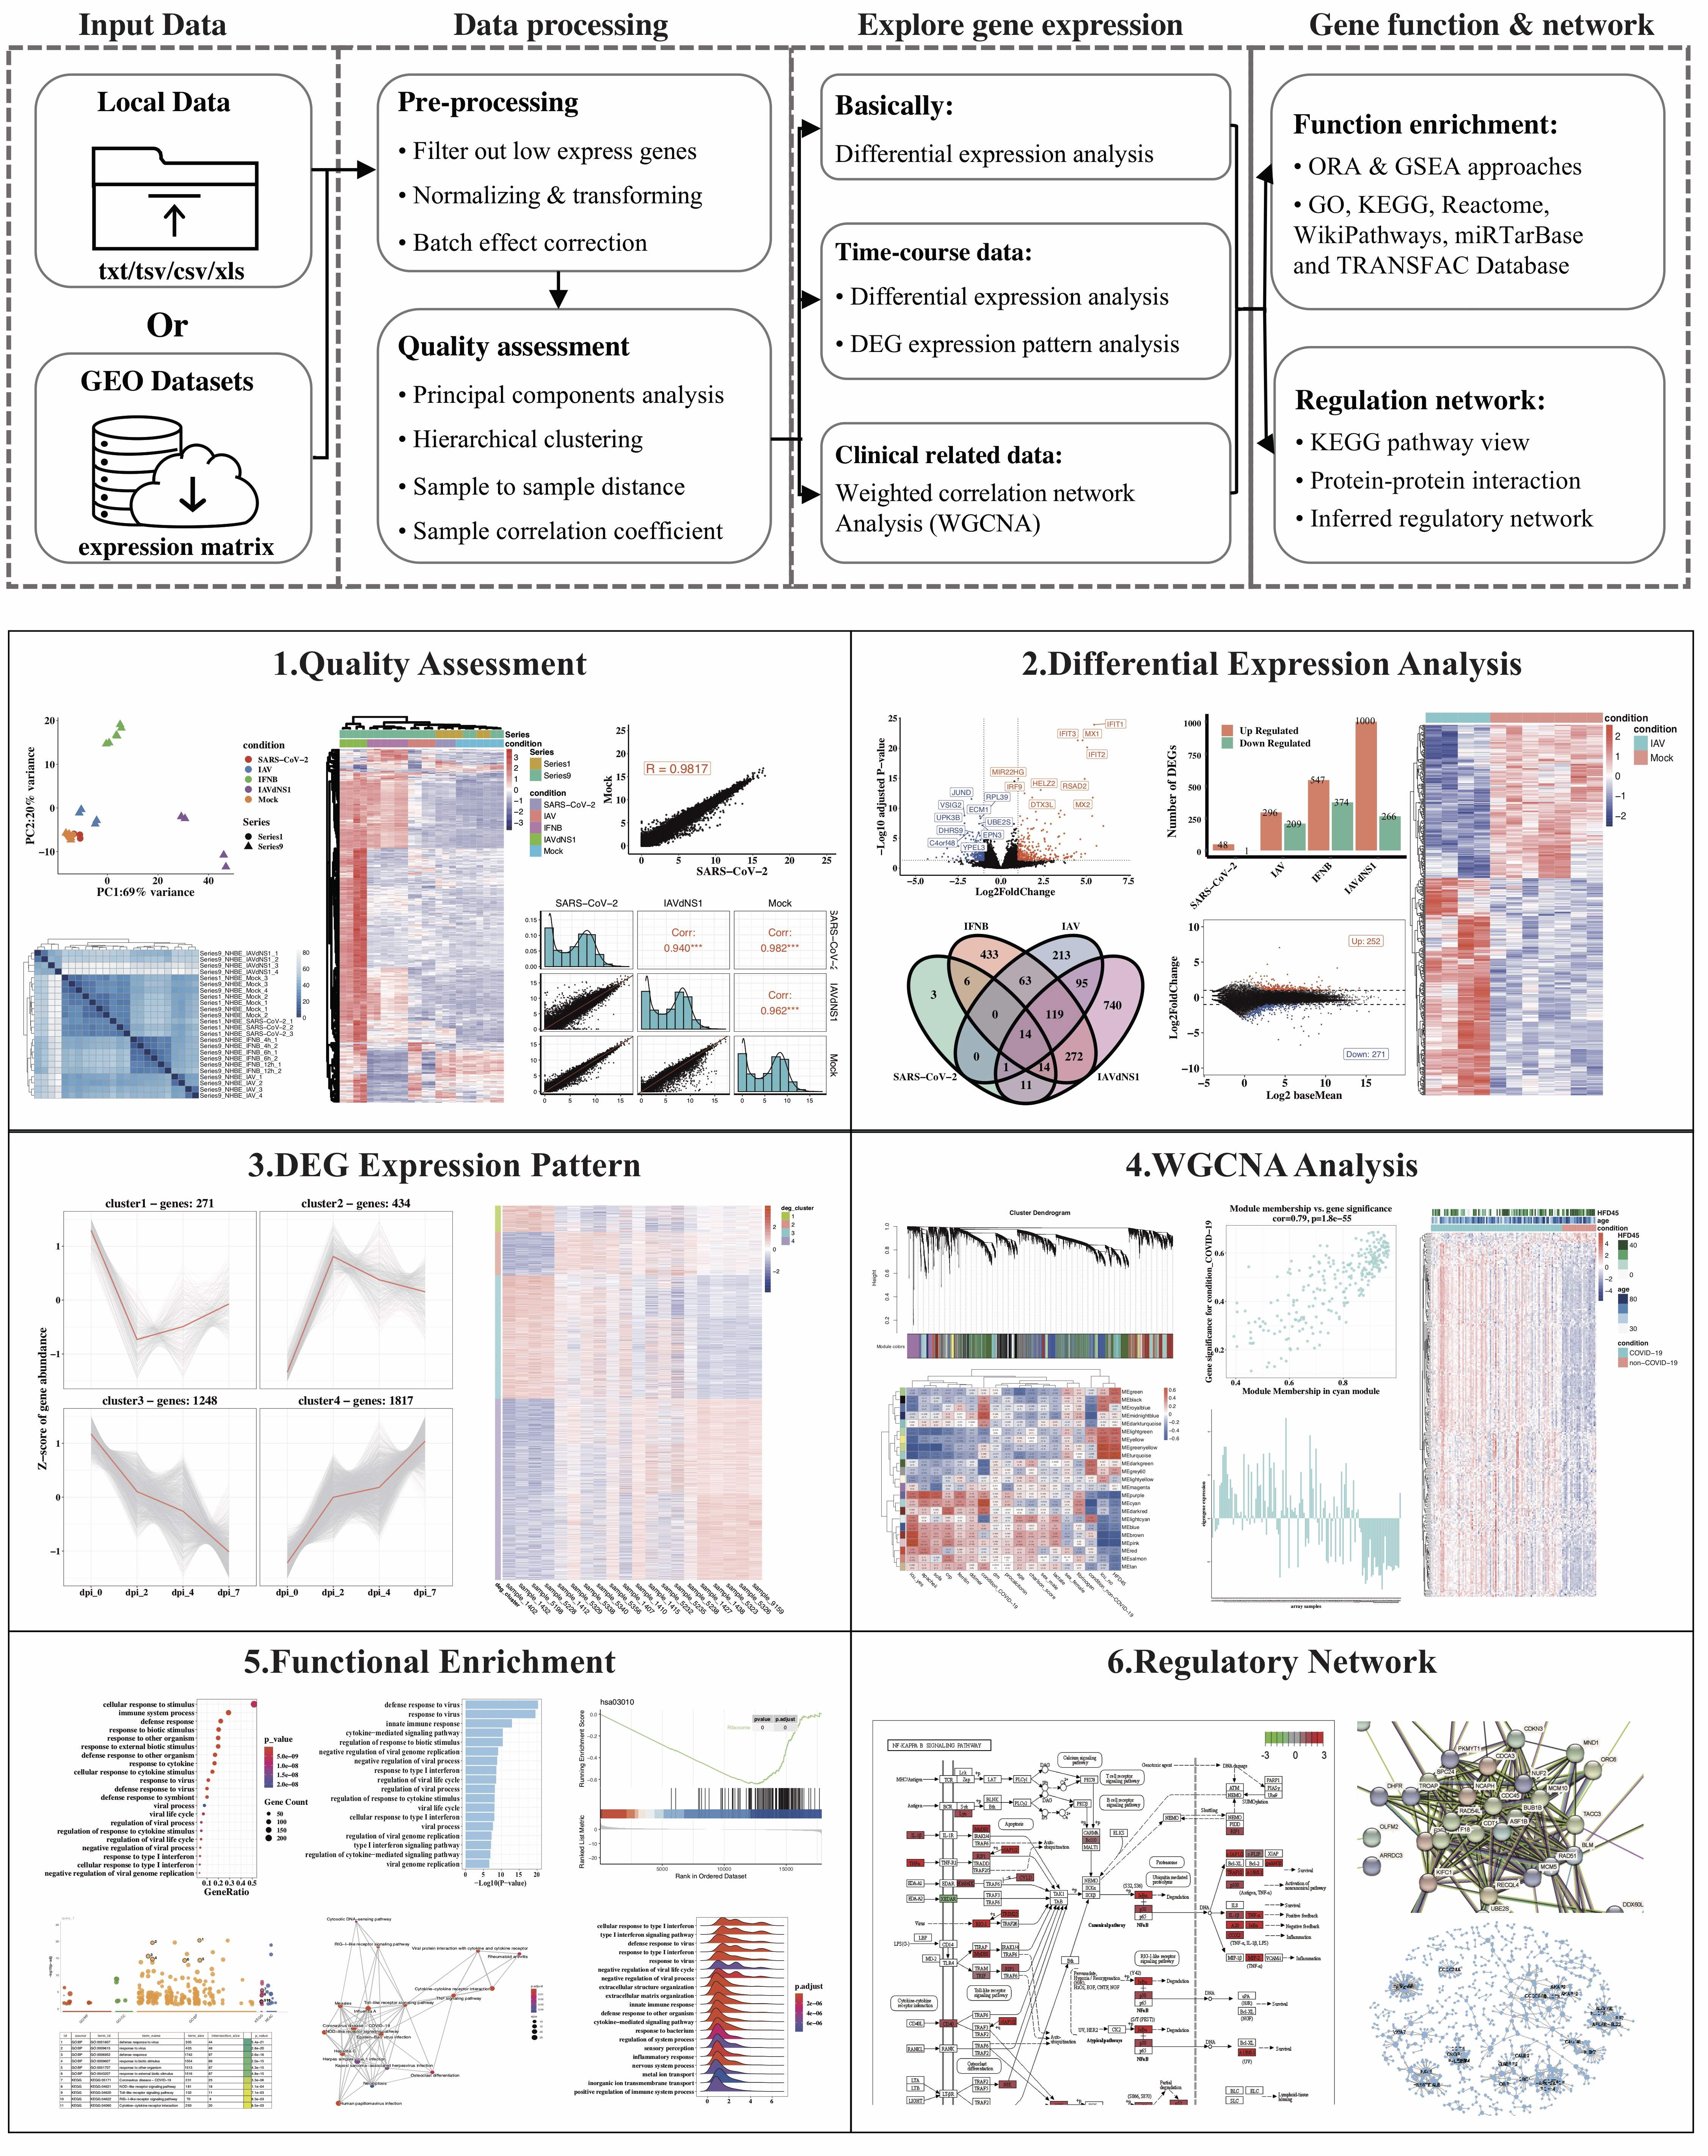
\includegraphics{images/workflow.jpg}

\hypertarget{intro}{%
\chapter{Introduction}\label{intro}}

\hypertarget{introduction}{%
\section{Introduction}\label{introduction}}

Motivation: RNA-sequencing (RNA-seq) has become the most commonly used tool in life science research for exploring whole transcript profiles. The advancement of next-generation sequencing has promoted a large amount of RNA-seq data. However, the popularity of bioinformatics lags far behind the generation of sequencing data, resulting in the inability of most researchers to analyze RNA-seq data. Although a large number of tools are currently available for RNA-seq analysis, data uploading, analysis, and visualization through an interactive interface are more acceptable to researchers than command-line codes.

Results: We designed an interactive RNA-seq analysis toolkit based on the R Shiny package, named QRAP (Quick RNA-seq Analysis Platform), which can easily accomplish RNA-seq data analysis and visualization through a user-friendly interface on the web page. As a comprehensive RNA-seq analysis tool, QRAP can support the analysis of publicly available and user-generated data, which include regular RNA-seq data, time-course RNA-seq data, and clinically relevant RNA-seq data, and provide functional annotation for approximately 500 species.

Availability and implementation: As an open source R package, QRAP can be freely accessed at \url{https://github.com/gsx-ucas/QRAP}.

\hypertarget{installation}{%
\section{Installation}\label{installation}}

\hypertarget{r-package}{%
\subsection{R package}\label{r-package}}

To install QRAP, R version 4.0 or greater is required. We also recommend installing R Studio.\\

\hypertarget{install-the-release-version-of-qrap}{%
\subsubsection{Install the release version of QRAP}\label{install-the-release-version-of-qrap}}

\begin{Shaded}
\begin{Highlighting}[]
\CommentTok{\# Enter commands in R (or R studio, if installed) }
\CommentTok{\# Install the remotes package install.packages(\textquotesingle{}devtools\textquotesingle{}) }
\NormalTok{devtools}\SpecialCharTok{::}\FunctionTok{install\_github}\NormalTok{(}\StringTok{"gsx{-}ucas/QRAP"}\NormalTok{)}
\end{Highlighting}
\end{Shaded}

\hypertarget{install-the-development-version-of-qrap}{%
\subsubsection{Install the development version of QRAP}\label{install-the-development-version-of-qrap}}

\begin{Shaded}
\begin{Highlighting}[]
\CommentTok{\# Enter commands in R (or R studio, if installed) }
\CommentTok{\# Install the remotes package install.packages(\textquotesingle{}devtools\textquotesingle{}) }
\NormalTok{devtools}\SpecialCharTok{::}\FunctionTok{install\_github}\NormalTok{(}\StringTok{"gsx{-}ucas/QRAP"}\NormalTok{, }\AttributeTok{ref =} \StringTok{"dev"}\NormalTok{)}
\end{Highlighting}
\end{Shaded}

\hypertarget{docker-image}{%
\subsection{Docker image}\label{docker-image}}

We provide docker images for QRAP via dockerhub. To pull the latest image using the command line:

\begin{Shaded}
\begin{Highlighting}[]
\CommentTok{\# Enter commands in shell}
\NormalTok{docker pull goushixue}\SpecialCharTok{/}\NormalTok{qrap}\SpecialCharTok{:}\NormalTok{latest}
\end{Highlighting}
\end{Shaded}

\hypertarget{get-started}{%
\section{Get started}\label{get-started}}

\hypertarget{launch-the-qrap-application-in-r-or-rstudio}{%
\subsection{Launch the QRAP application in R or Rstudio}\label{launch-the-qrap-application-in-r-or-rstudio}}

\begin{Shaded}
\begin{Highlighting}[]
\FunctionTok{library}\NormalTok{(QRAP) }\CommentTok{\# loading the QRAP library to R environment}
\FunctionTok{startQRAP}\NormalTok{() }\CommentTok{\# launch the QRAP application to web browser}
\end{Highlighting}
\end{Shaded}

Then you would get the link to activate your browser:\\
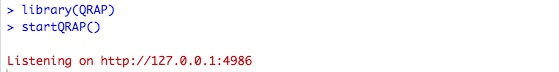
\includegraphics{images/launch_R.jpeg}\\
Use the link \url{http://127.0.0.1:4986} to access the interactive analysis interface. Note that the port (4986) should change to yours.\\

\hypertarget{launch-the-qrap-application-by-docker-image-in-shell}{%
\subsection{Launch the QRAP application by docker image in shell}\label{launch-the-qrap-application-by-docker-image-in-shell}}

\begin{Shaded}
\begin{Highlighting}[]
\NormalTok{docker run  }\SpecialCharTok{{-}}\NormalTok{p }\DecValTok{3838}\SpecialCharTok{:}\DecValTok{3838}\NormalTok{ goushixue}\SpecialCharTok{/}\NormalTok{qrap }\CommentTok{\# use the 3838 port }
\end{Highlighting}
\end{Shaded}

Then you would get the output like this:\\
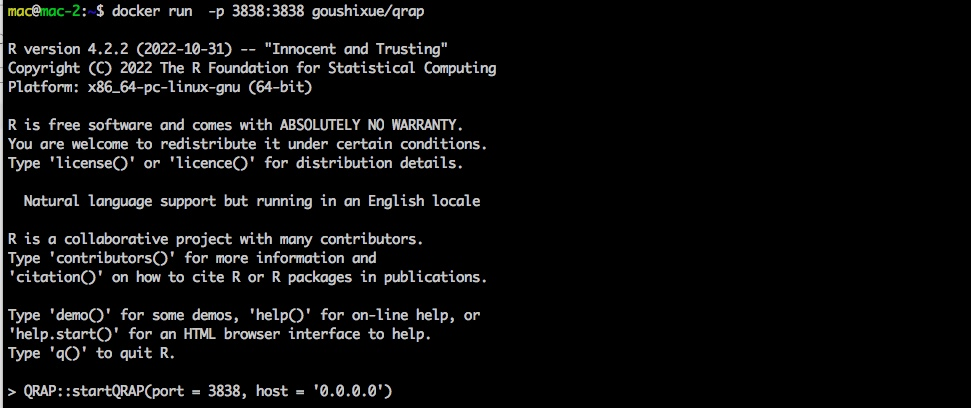
\includegraphics{images/launch_docker.jpeg}\\
Use the link \url{http://localhost:3838/} to access the interactive analysis interface.\\

\hypertarget{access-the-interactive-analysis-interface}{%
\subsection{Access the interactive analysis interface}\label{access-the-interactive-analysis-interface}}

Just start your analysis by clicking, clicking, clicking\ldots{}\\
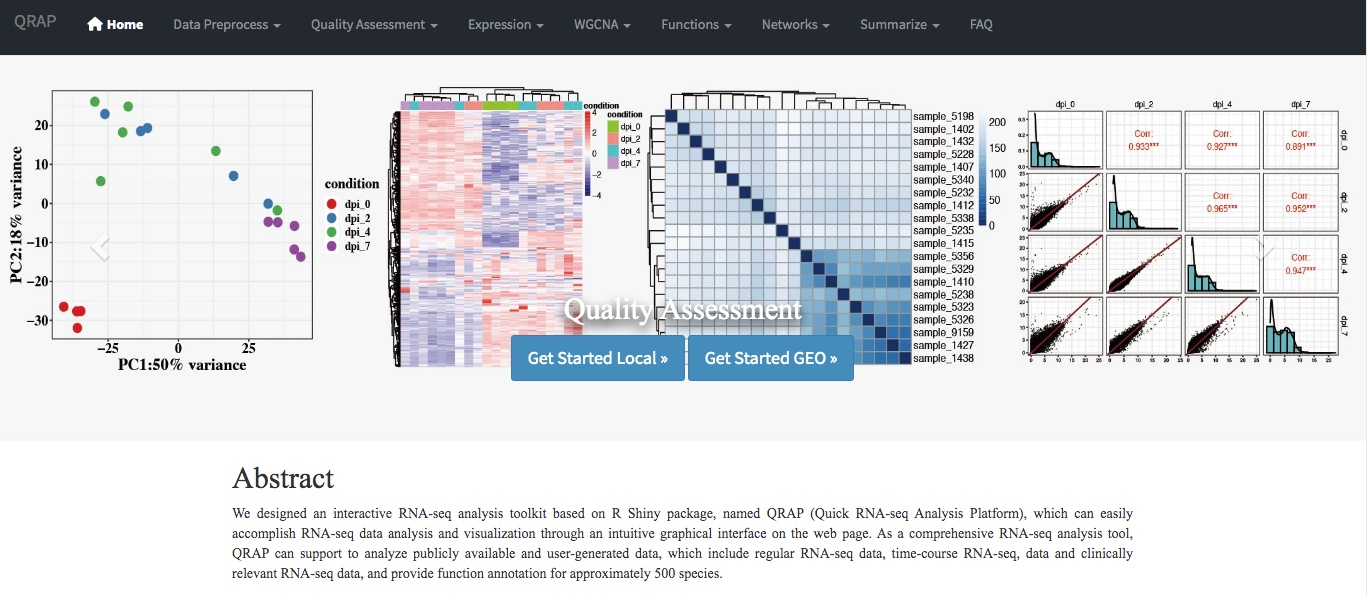
\includegraphics{images/launch_interface.jpeg}\\

\hypertarget{data-input-and-pre-processing}{%
\chapter{Data input and pre-processing}\label{data-input-and-pre-processing}}

\hypertarget{data-input}{%
\section{Data input}\label{data-input}}

QRAP can support to analyze publicly available and user-generated data. There are two action buttons, `Get Started Local' and `Get Started GEO', can activate corresponding data upload and processing pipeline.

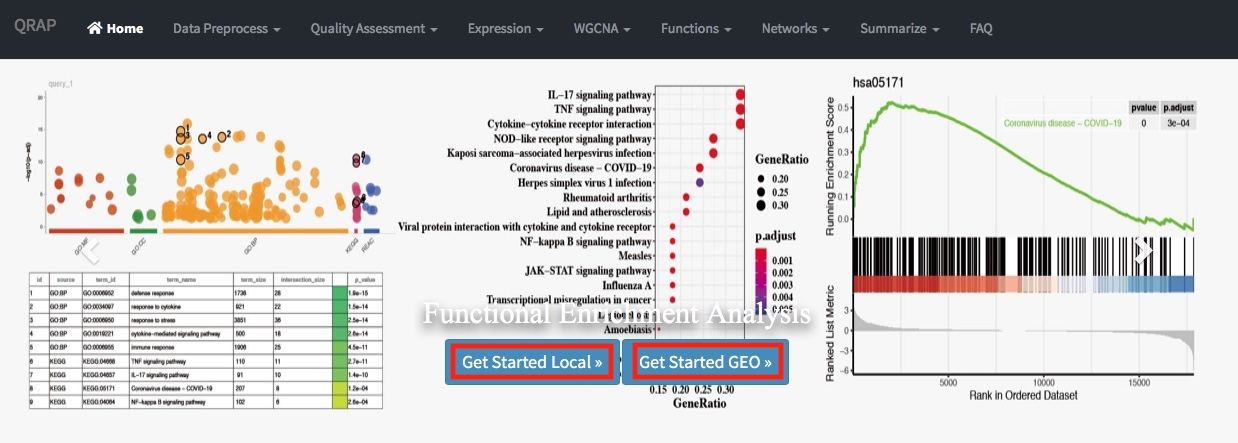
\includegraphics{images/start_button.jpeg}

\hypertarget{upload-local-file}{%
\subsection{Upload local file}\label{upload-local-file}}

For user generated local files, click the `Get Started Local' button to enter the data upload page. Users need to upload a read-count matrix, in which rows represent the genes and columns represent the samples, while the contents represent the gene expression values of given sample

\textbf{\emph{Parameters in this section:}}\\
- Choose input file: browser and upload the expression matrix file, accept .csv/.tsv/.tab/.txt format.\\
- First row as header ? This means use the first row of the expression matrix as column names, often is samples names.\\
- First column as rownames ? This means use the first column of the expression matrix as row names, often is gene names.\\

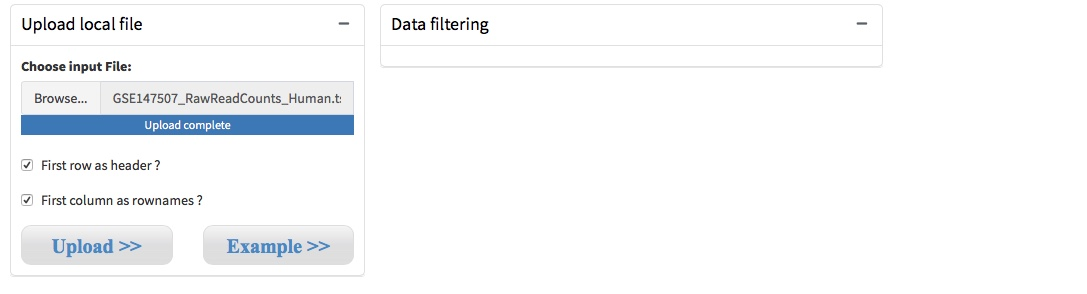
\includegraphics{images/upload_local_file.jpeg}

After select the local files and set the parameters, click the `Upload' button to preview the expression matrix.

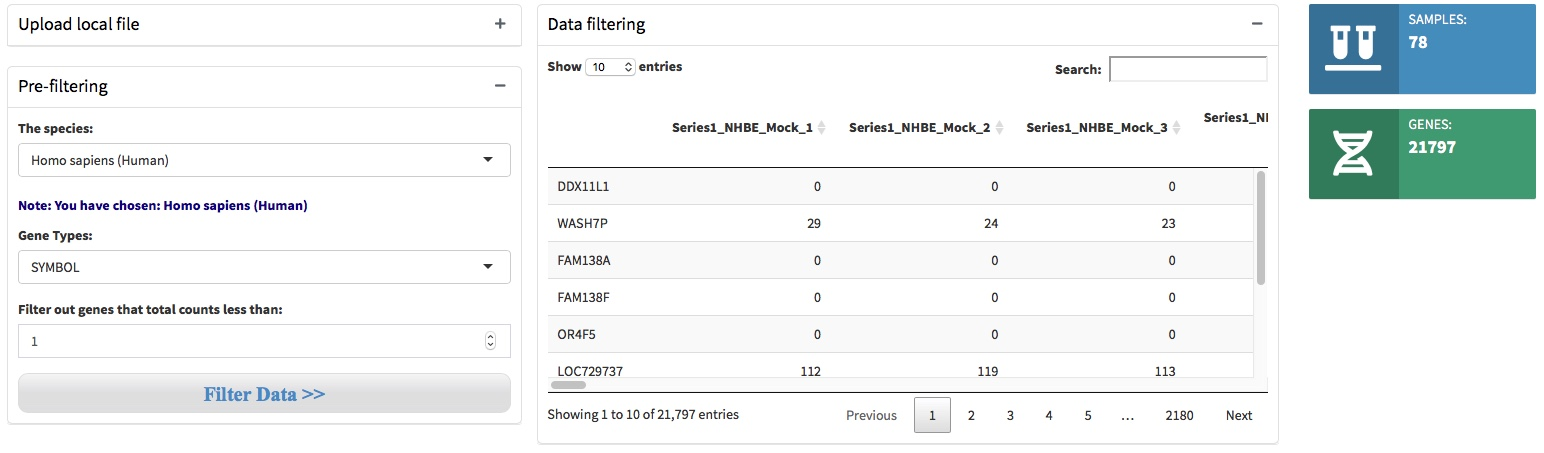
\includegraphics{images/local_expression_preview.jpeg}

Click `Example' will upload the example dataset internal, transcriptomes of SARS-Cov-2 infected normal human bronchial epithelial cells (GSE147507).

\hypertarget{pull-down-geo-datasets}{%
\subsection{Pull down GEO datasets}\label{pull-down-geo-datasets}}

The Gene Expression Omnibus (GEO) is a public repository that archives and freely distributes comprehensive sets of microarray, next-generation sequencing, and other forms of high-throughput functional genomic data submitted by the scientific community.

For GEO datasets, users need to input an accession number to query the gene expression matrix through GEOquery. After you input the GEO Acession Number and active the `Download matrix' button, We will download the value matrix tables within GDSxxx or supplementary files within GSExxx, these files will store in the working directory of the R project you created.\\
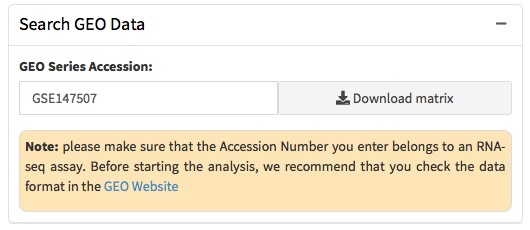
\includegraphics{images/search_geo_dataset.jpeg}\\

When the files download accomplished, there will show the download files name in the Parameter setting panel, and you should select file(s) that contain interested gene expression matrix and active the `Loading GEO' button to preview the matrix.\\
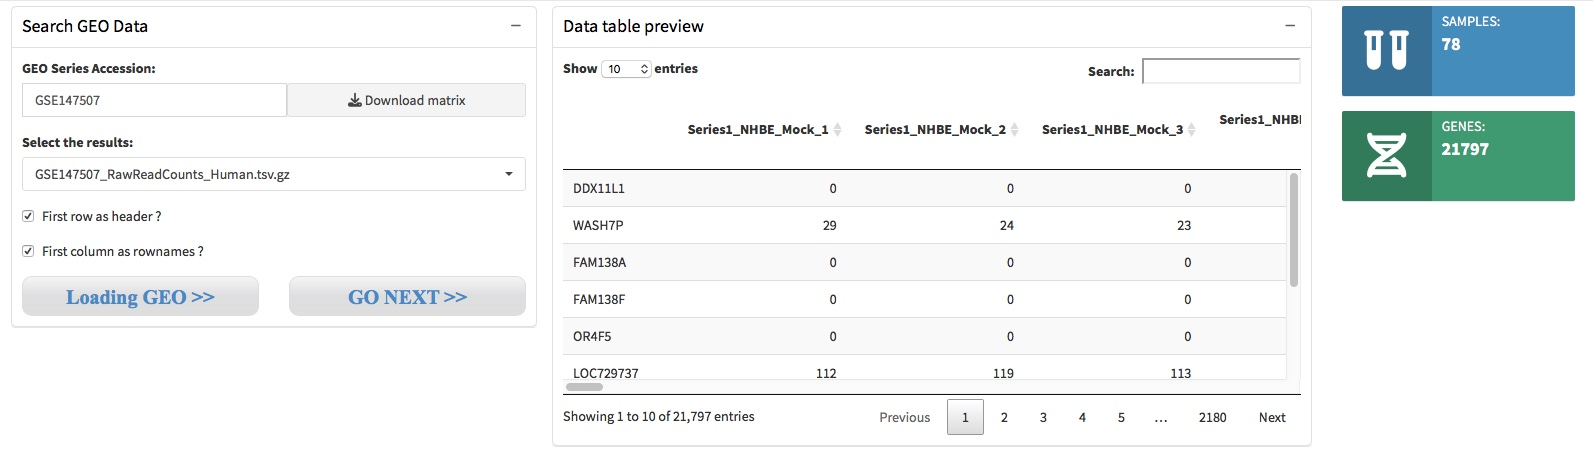
\includegraphics{images/geo_preview_single.jpeg}\\
Please Note that if the files are in a tar archive format, such as htseq-count generated results, these files will contain Gene ID and Gene Expression Value of each sample, respectively. Therefore, you need to provid the column number of the Gene ID and Gene Expression Value to help merge the files to generate an analysis ready gene expression matrix.

\begin{itemize}
\tightlist
\item
  Step 1. Choose a single file, and leave the `First row as header' and `First column as rownames' unchecked, then click the button `Loading GEO' to preview what the file contained.\\
  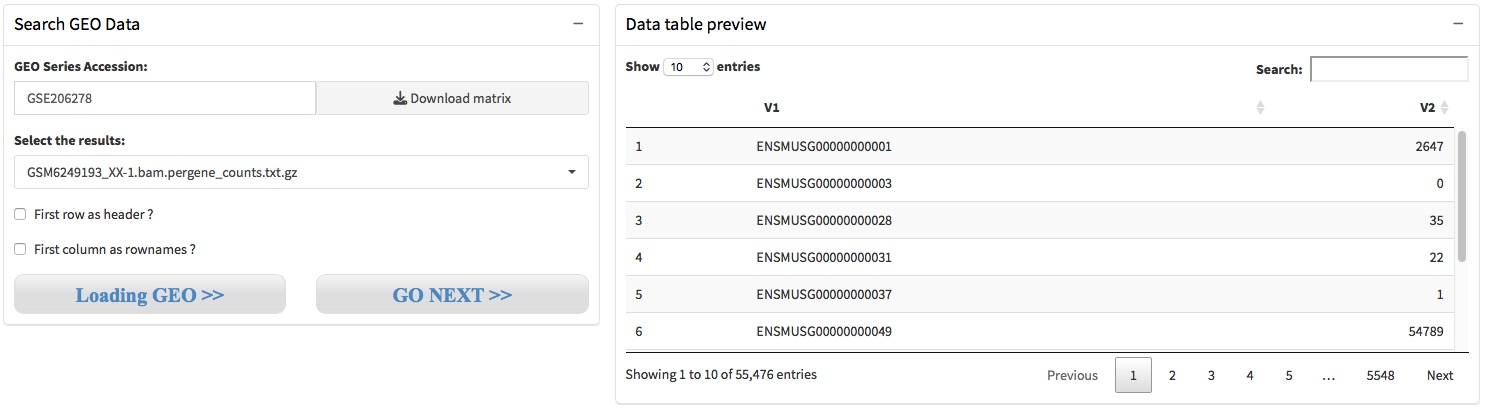
\includegraphics{images/geo_preview_multiple_setp1.jpeg}
\item
  Step 2. Choose all or interested files, set the column number of geneID and readCounts, then click the button `Loading GEO' to generate and preview the analysis ready expression matrix.\\
  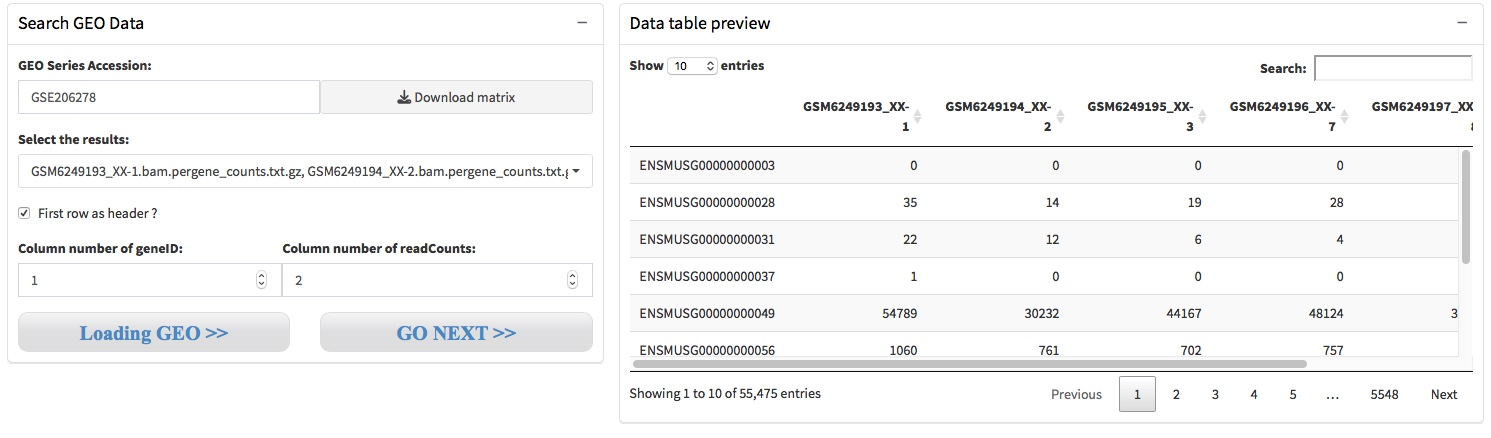
\includegraphics{images/geo_preview_multiple_setp2.jpeg}
\end{itemize}

\hypertarget{data-pre-filtering}{%
\section{Data pre-filtering}\label{data-pre-filtering}}

QRAP starts with a read-counts matrix or GEO accession number, and then filters out low expression genes under an given threshold. We then specify the organisms and filtered out low expression genes.\\
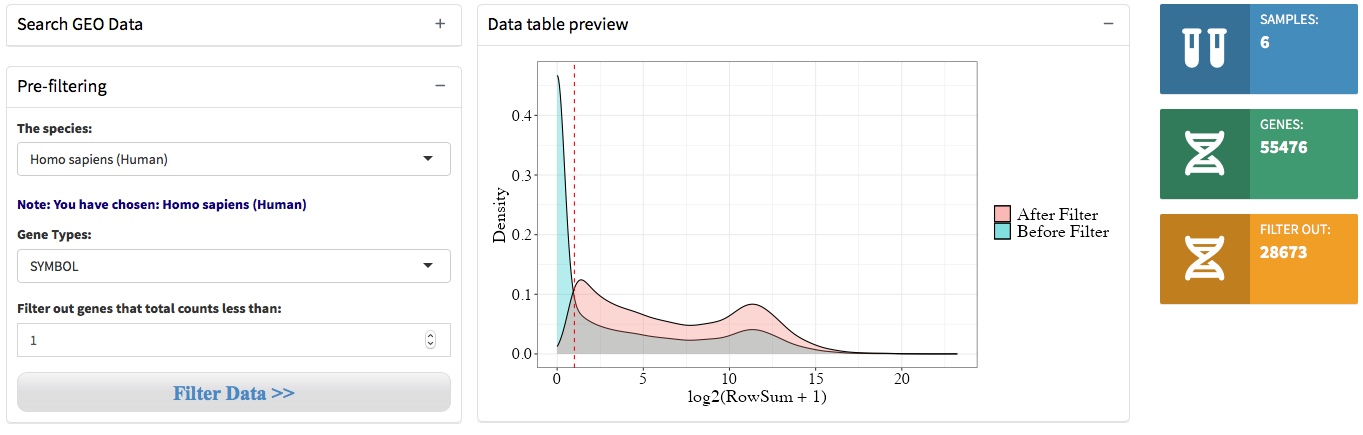
\includegraphics{images/prefiltering.jpeg}

\hypertarget{note-the-gene-types}{%
\subparagraph*{Note the Gene Types:}\label{note-the-gene-types}}
\addcontentsline{toc}{subparagraph}{Note the Gene Types:}

\begin{longtable}[]{@{}lll@{}}
\toprule()
SYMBOL & ENSEMBL & ENTREZID \\
\midrule()
\endhead
GAPDH & ENSG00000111640 & 2597 \\
TP53 & ENSG00000141510 & 7157 \\
\bottomrule()
\end{longtable}

\hypertarget{design-table-formula}{%
\section{Design table \& formula}\label{design-table-formula}}

A DESeqDataSet object must have an associated design formula. The design formula expresses the variables which will be used in modeling. QRAP will automatically produces an dataframe that contain sample names in the first column and condition variables in the second column. The condition column was simply generated by deleting the replicates numbers (eg. -1, -2, -3). User can download this design table by the button where the arrow indicated.
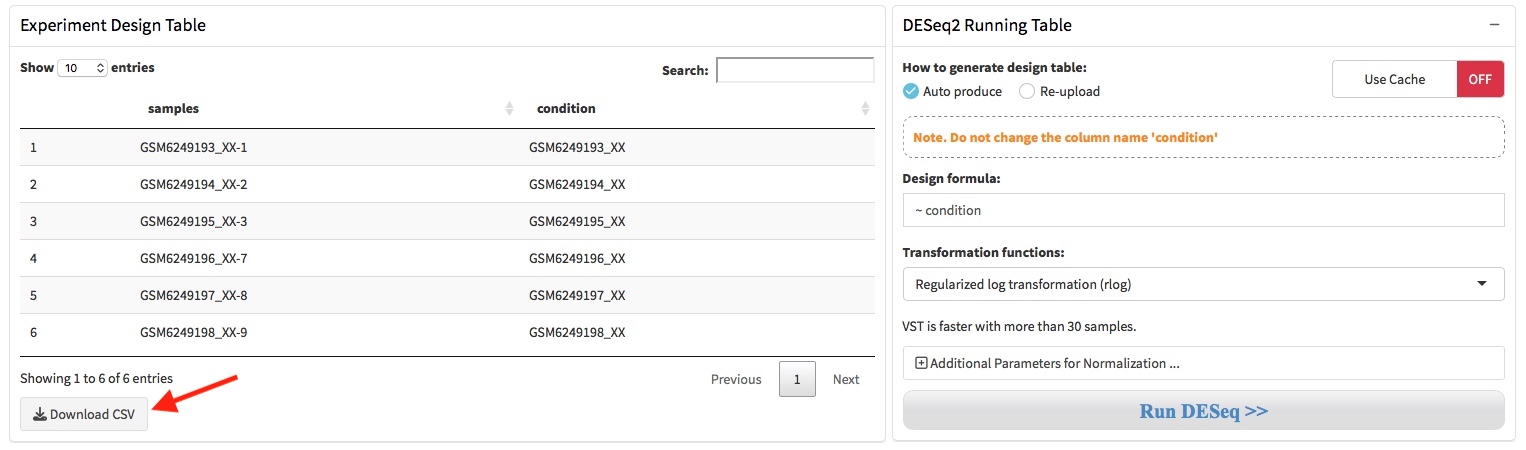
\includegraphics{images/design_table-auto.jpeg}
If the condition variables in the second column were not produced correctly, user should adjust it manually in Microsoft Excel and save it as .csv format file. Then, user need choose the `Re-upload' option where the arrow shows and re-upload the corrected design table through the file upload box.
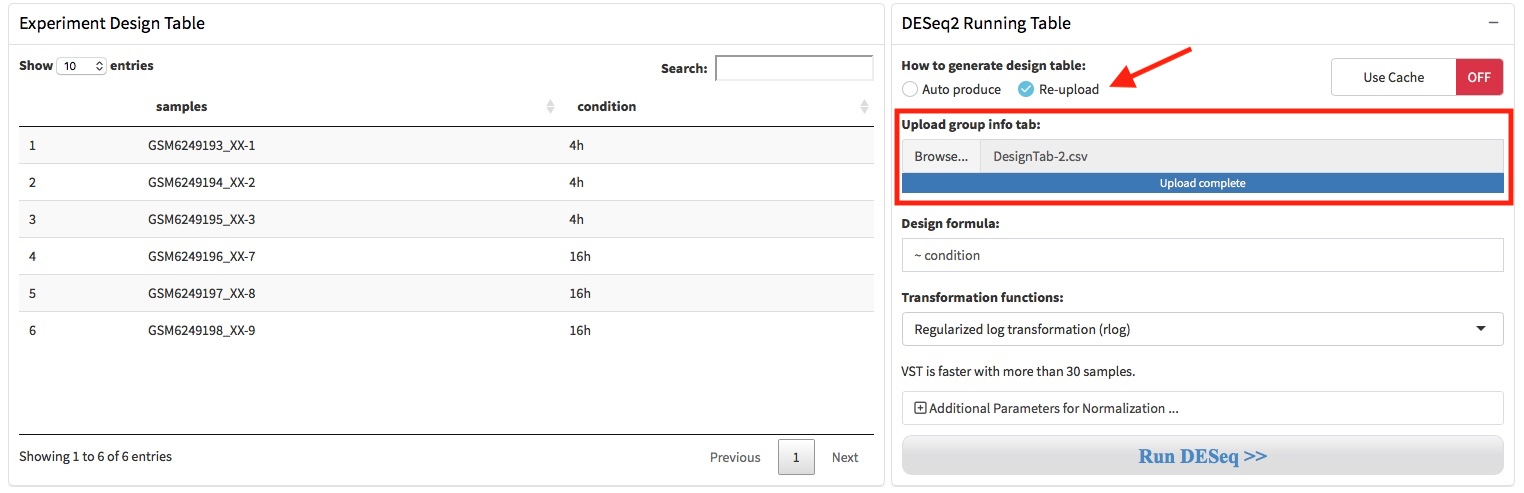
\includegraphics{images/design_table-reupload.jpeg}

The formula should be a tilde (\textasciitilde) followed by the variables, and the is used to estimate the dispersions and to estimate the log2 fold changes of the model. The transformation functions can be specified as rlog (regularized logarithm) and vst (variance stabilizing transformations).

\hypertarget{batch-effect-correction}{%
\section{Batch effect correction}\label{batch-effect-correction}}

If there is unwanted variation present in the data (e.g.~batch effects) it is always recommend to correct for this. The batch effects can be accommodated in DESeq2 by including in the design any known batch variables, and estimated by functions ComBat in sva (Leek 2014) or removwBatchEffect in limma (Matthew et al.~2015).
1. For performing batch effect correction, the two factor variables batch and condition should be columns of the design table.
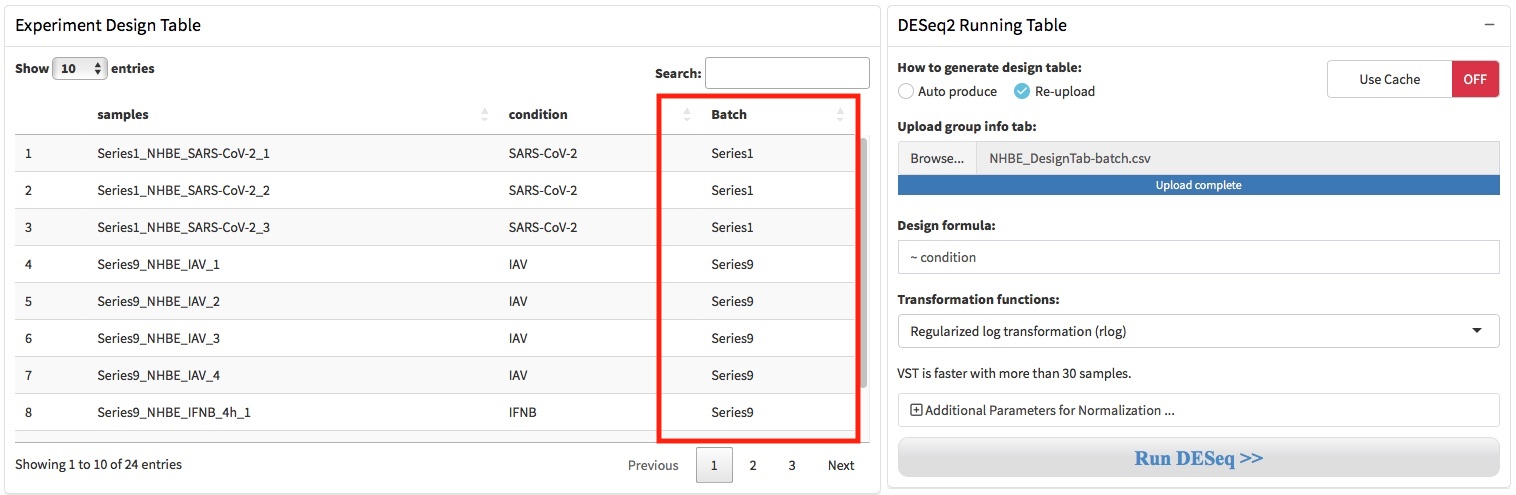
\includegraphics{images/design_table-batch.jpeg}
2. Setting the batch correction parameters by click ``Additional Parameters \ldots{}'' button. Two functions were provide to perform batch correction, ComBat in sva or removwBatchEffect in limma.
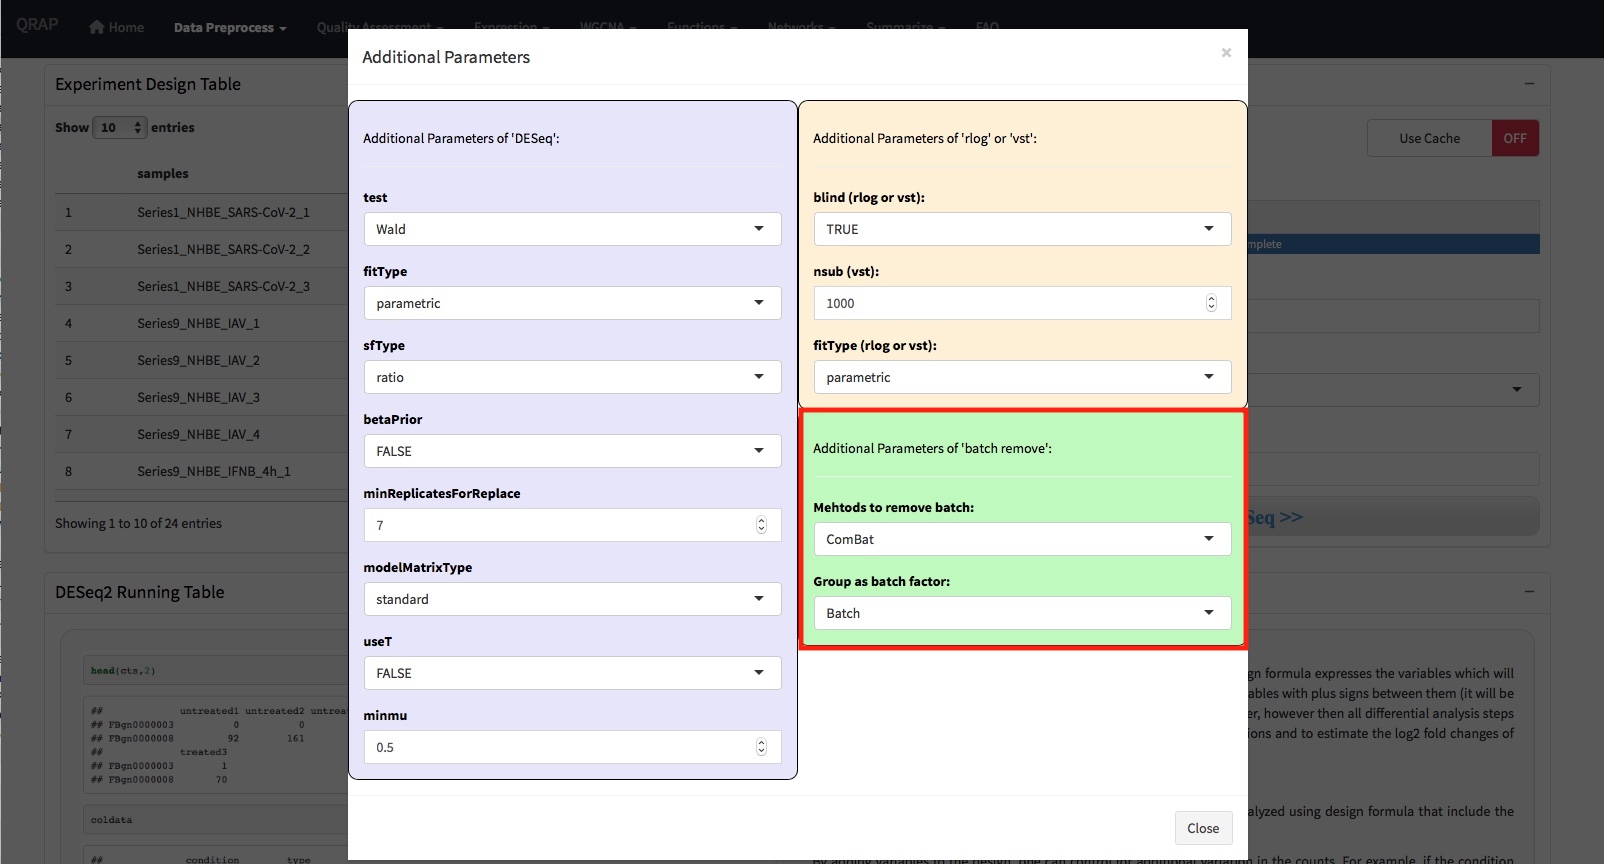
\includegraphics{images/batch-remove-parameter.jpeg}

\hypertarget{data-quality-exploring}{%
\chapter{Data quality exploring}\label{data-quality-exploring}}

In biological experiments, it is often necessary to set up technical and biological repetition to avoid accidental variation affecting the results. RNA-seq usually sets 3-5 biological repeats, so it is necessary to confirm the quality of biological repetitions and determine that the sequencing data can truly reflect the transcriptome changes across experimental conditions. Principal components analysis (PCA), hierarchical clustering heatmap, sample to sample heatmap and sample correlation coefficient was the most used method to assess the sequencing data quality, which can identify bad sample replicates and batch effects.

\hypertarget{principal-component-analysis-pca}{%
\section{Principal component analysis (PCA)}\label{principal-component-analysis-pca}}

Principal component analysis (PCA) is a mathematical algorithm that reduces the dimensionality of the data while retaining most of the variation in the data set1. It accomplishes this reduction by identifying directions, called principal components, along which the variation in the data is maximal. By using a few components, each sample can be represented by relatively few numbers instead of by values for thousands of variables. Samples can then be plotted, making it possible to visually assess similarities and differences between samples and determine whether samples can be grouped.

As shown in the screenshot below, left panel provides the parameters to perform PCA and visualize the results, middle panel will show the visualization results, and right panel provides the control of the width and height of figure.

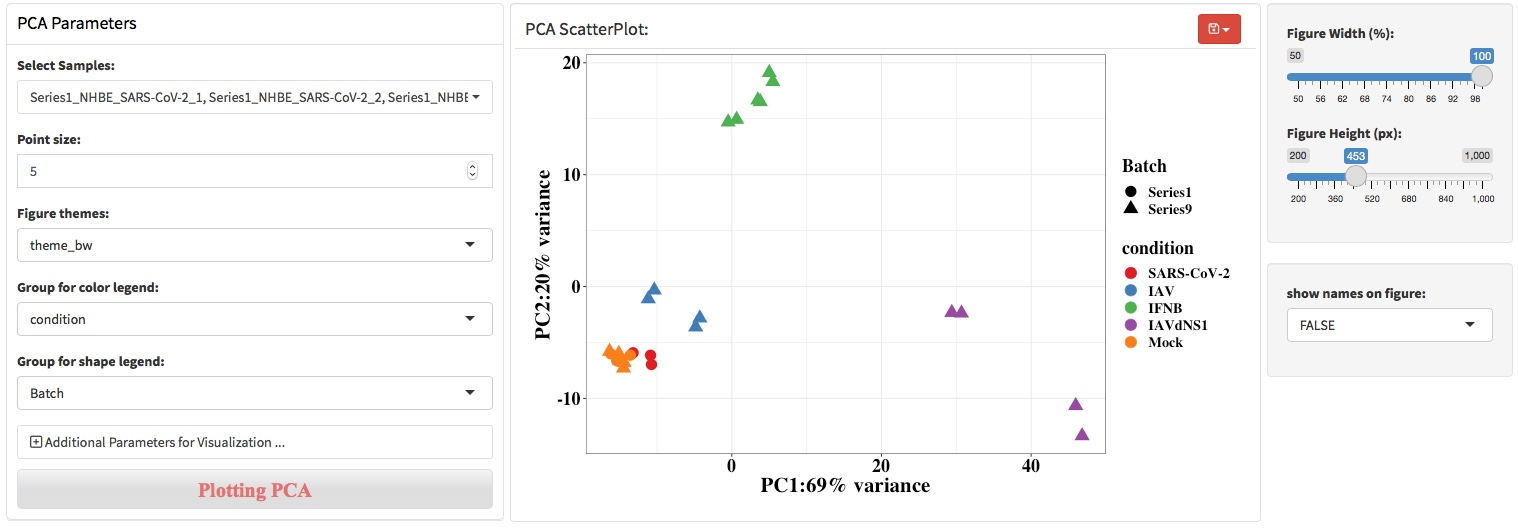
\includegraphics{images/quality_pca.jpeg}

For users with programming skills, ggplot2 codes can be added to modify the figure layer directly. Just note that do not add plus sign (+) at the beginning of the first line codes.

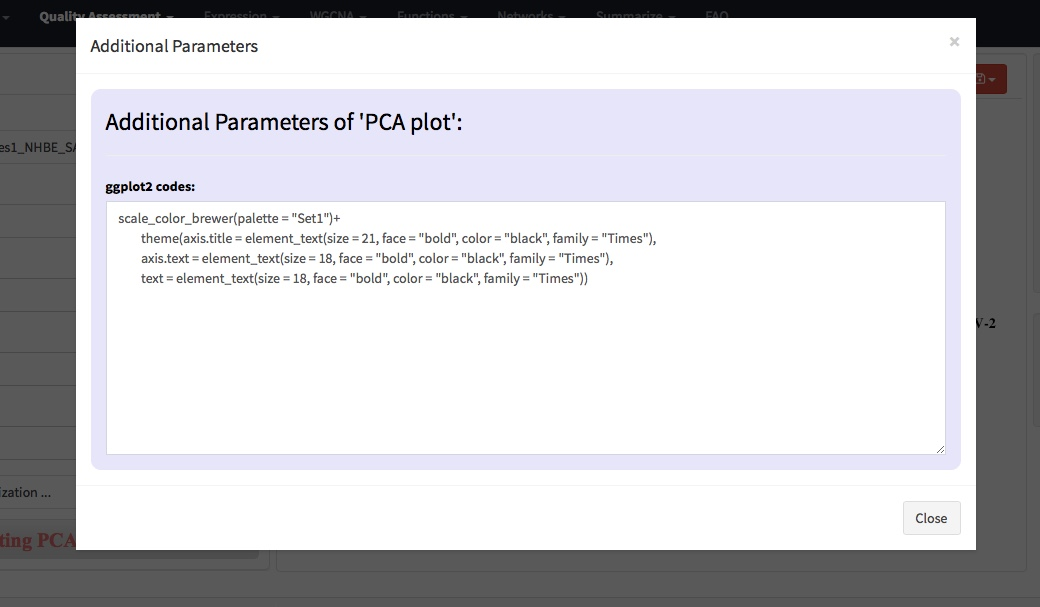
\includegraphics{images/quality_pca_add.jpeg}

\hypertarget{hierarchical-clustering}{%
\section{Hierarchical clustering}\label{hierarchical-clustering}}

Hierarchical clustering analysis is an algorithm that groups similar objects into groups called clusters. The endpoint is a set of clusters, where each cluster is distinct from each other cluster, and the objects within each cluster are broadly similar to each other. In RNA-seq, the objects can be samples or genes. HCA is often combined with heatmap to show the cluster of samples in the column and genes in the rows.

The agglomeration algorithm of hierarchical clustering combines the two most similar data points (genes or samples) of all data points by calculating the similarity between the two types of data points, and iterates this process repeatedly. To put it simply, the agglomeration algorithm of hierarchical clustering is to determine the similarity between each category of data points and all data points by calculating the distance between them. The smaller the distance, the higher the similarity. And the two nearest data points or categories are combined to generate a cluster tree.

To perform hierarchical clustering analysis, users should specify how many genes to used for this analysis. Typically, top 500 or 1000 most high variable genes will be used for clustering genes and samples.

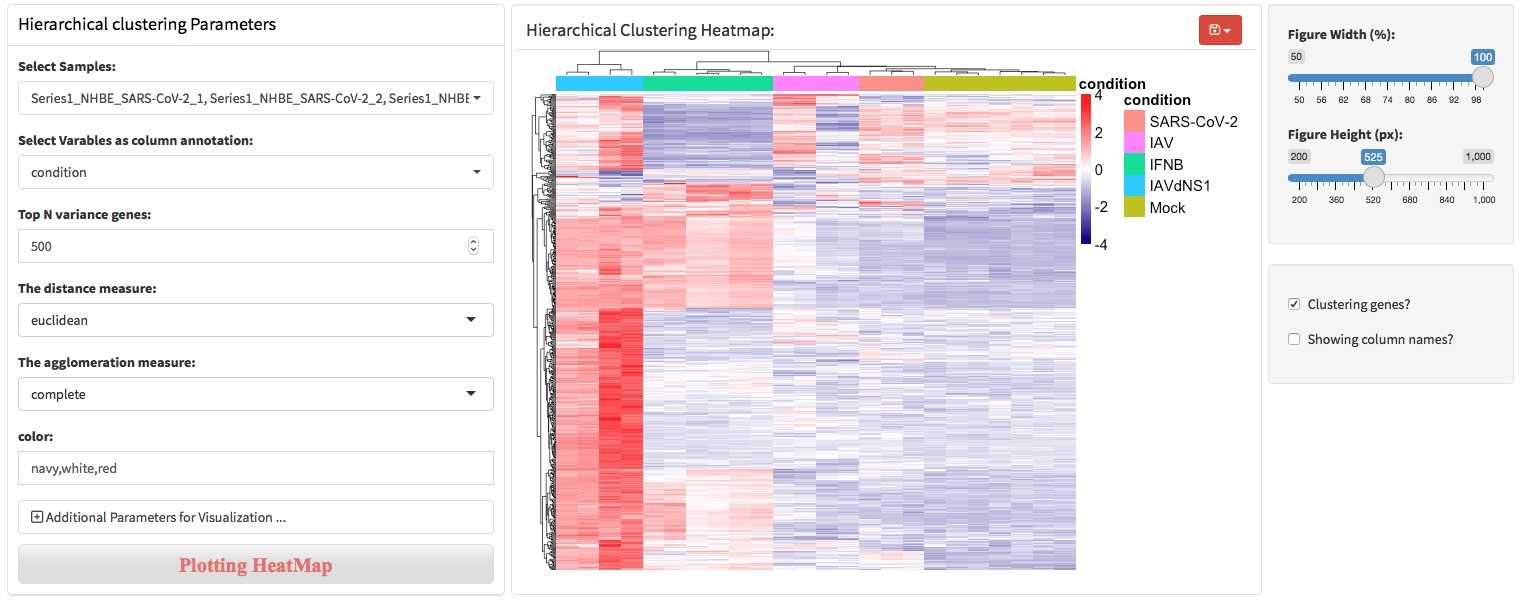
\includegraphics{images/quality_hca.jpeg}
To change colors of the heatmap, users can enter three colors separated by comma. The colors entered will be used to generate an continuous color vector to specify the colors of heatmap. For example, to generate a heatmap colored by `green,black,red'.

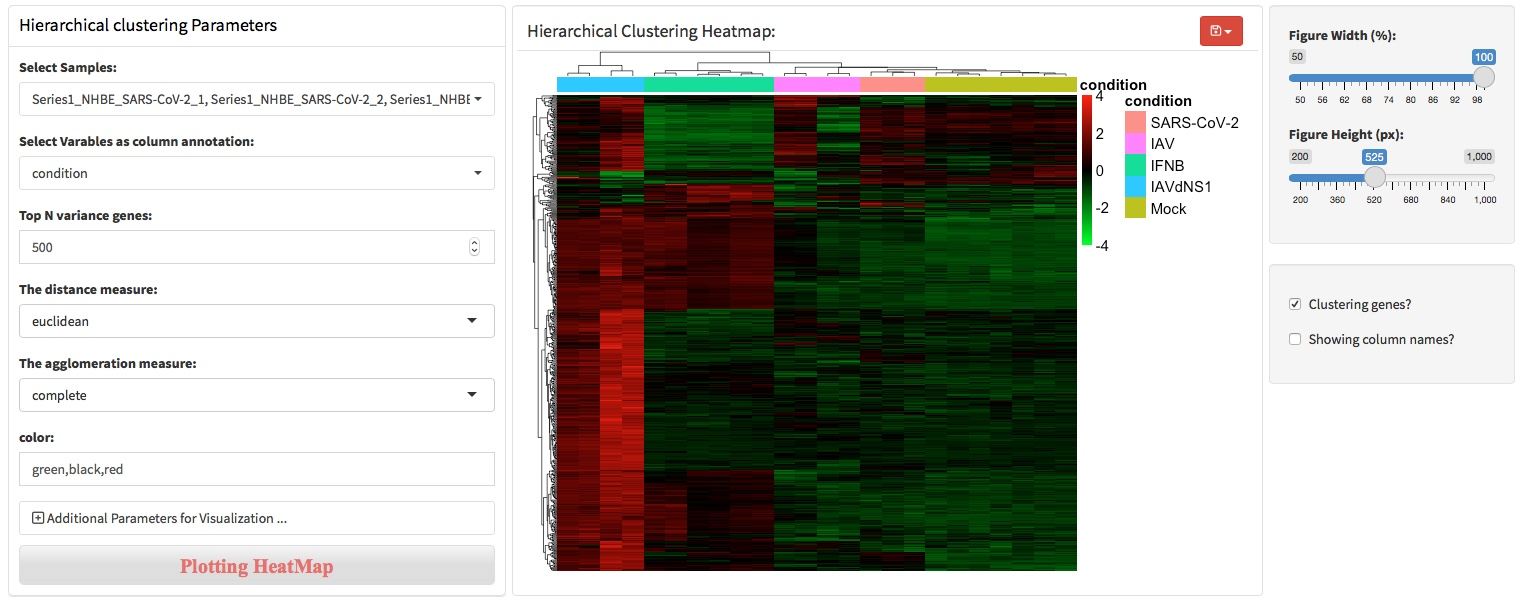
\includegraphics{images/quality_hca_color.jpeg}

To divide the heatmap based on the hierarchical clustering, users can specify the parameters throung `Additional parameters \ldots{}'.

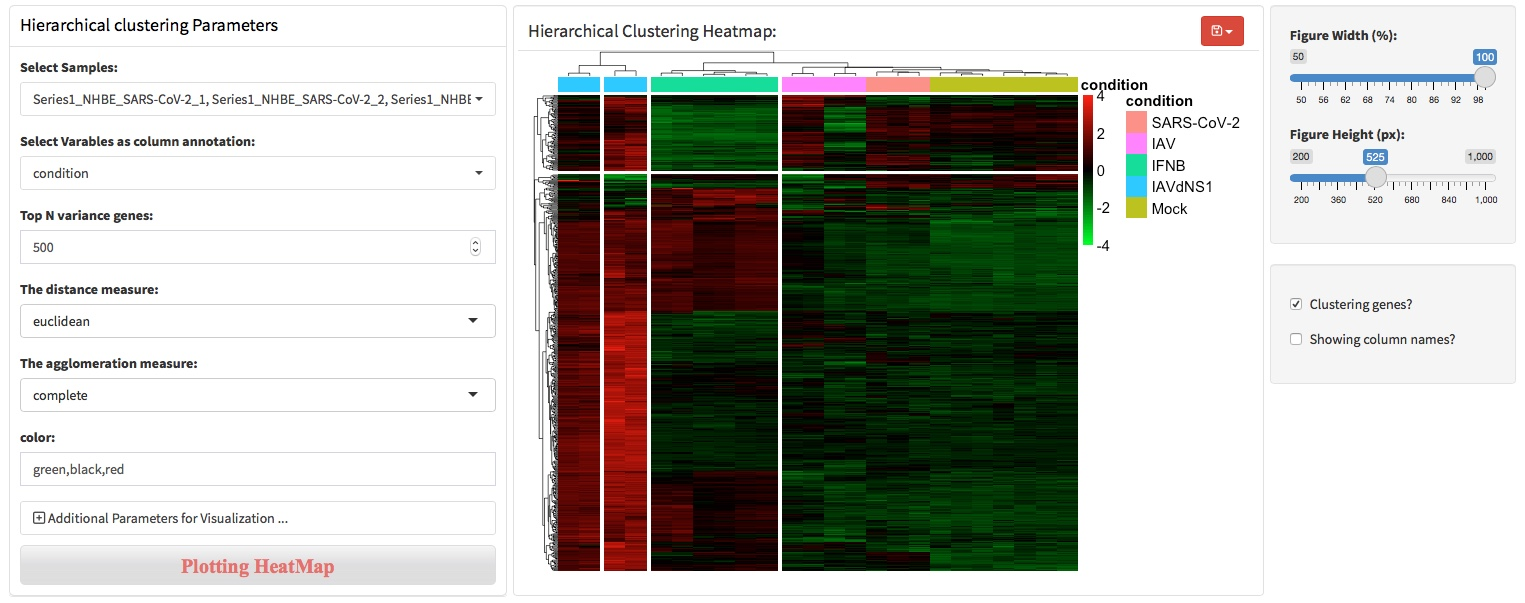
\includegraphics{images/quality_hca_split.jpeg}

\hypertarget{sample-to-sample-distance}{%
\section{Sample-to-sample distance}\label{sample-to-sample-distance}}

Sample-to-sample distance (SSD) is another method to assess sequencing and sample replicates quality based on calculated distance between samples. SSDA calculated similarity between samples based on distance metrics, which specify how the distance between the input samples. A commonly used approach for measuring sample distance in RNA-seq data is to use Euclidean distance.

SSD can elucidate samples distance in the high-dimensional space. In RNA-seq data, each gene is a dimension, so the data has tens of thousands of dimensions. SSD uses Euclidean distance to elucidate samples distance in the high-dimensional space, which helps to understand the relationship of samples across experimental conditions or sample replicates. The heatmap clusters samples with similar distances, which makes the results easier to interpret.

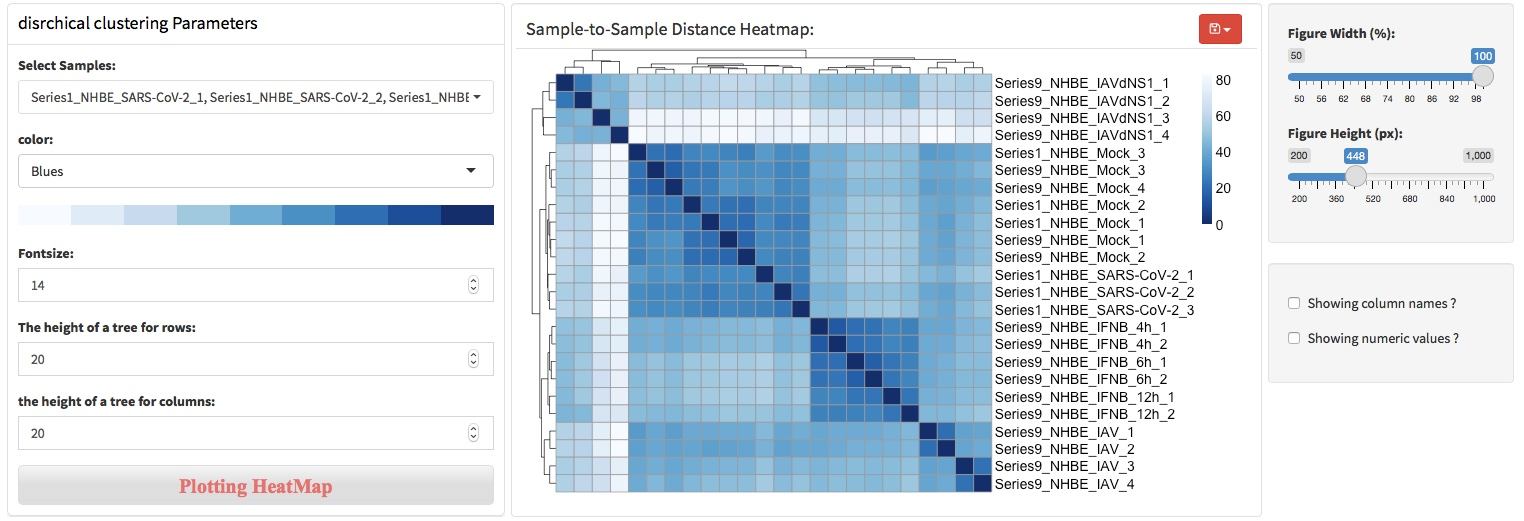
\includegraphics{images/quality_ssd.jpeg}

\hypertarget{sample-correlation-coefficient}{%
\section{Sample correlation coefficient}\label{sample-correlation-coefficient}}

The correlation coefficient is a statistical measure of the strength of the relationship between the relative movements of two variables. The values range between -1.0 and 1.0. A calculated number greater than 1.0 or less than -1.0 means that there was an error in the correlation measurement. A correlation of -1.0 shows a perfect negative correlation, while a correlation of 1.0 shows a perfect positive correlation. A correlation of 0.0 shows no linear relationship between the movement of the two variables.

Correlation statistics can be used in RNA-seq for assessing data quality. For example, a correlation coefficient could be calculated to determine the correlation between sample replicates, which indicate the biological replication quality of samples. Another example, a correlation coefficient between conditions, such as treatment group and WT control, could indicate the treatment effects.

Three visualization methods were provided in this section, heatmap, scatterplot and pairs.penels.

\begin{itemize}
\item
  heatmap
  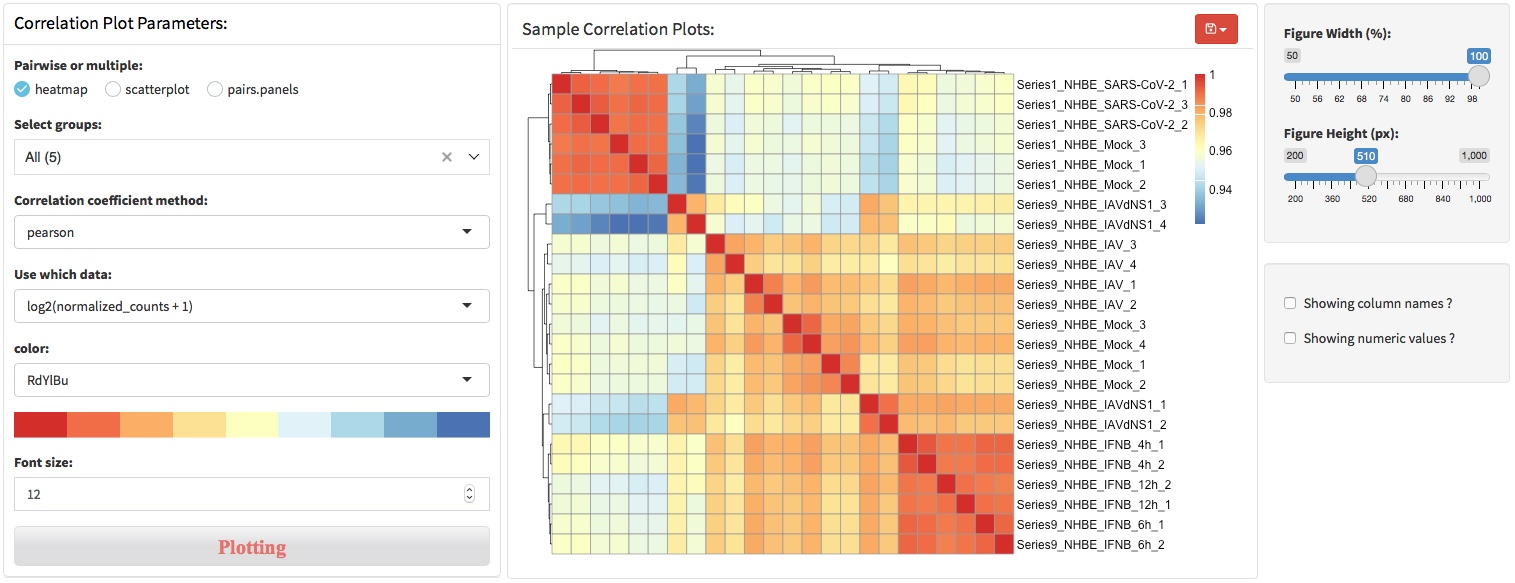
\includegraphics{images/quality_correlation.jpeg}
\item
  scatterplot
  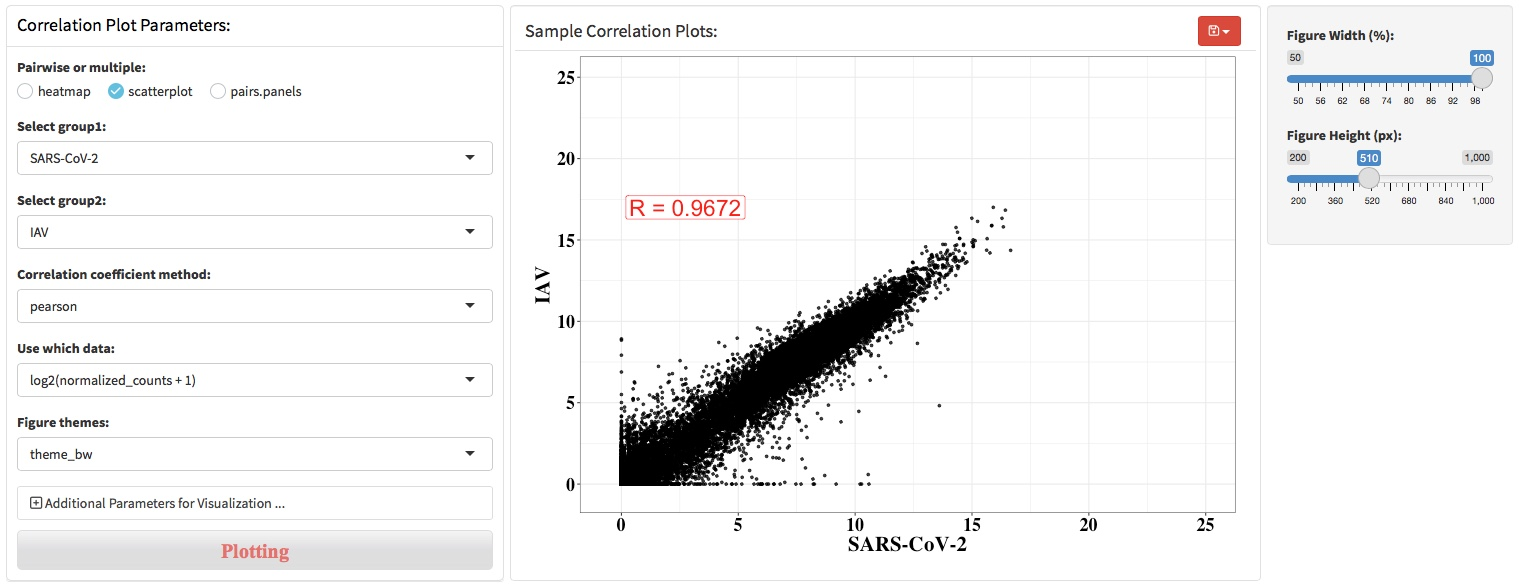
\includegraphics{images/quality_correlation-scatter.jpeg}
\item
  pairs.penels
  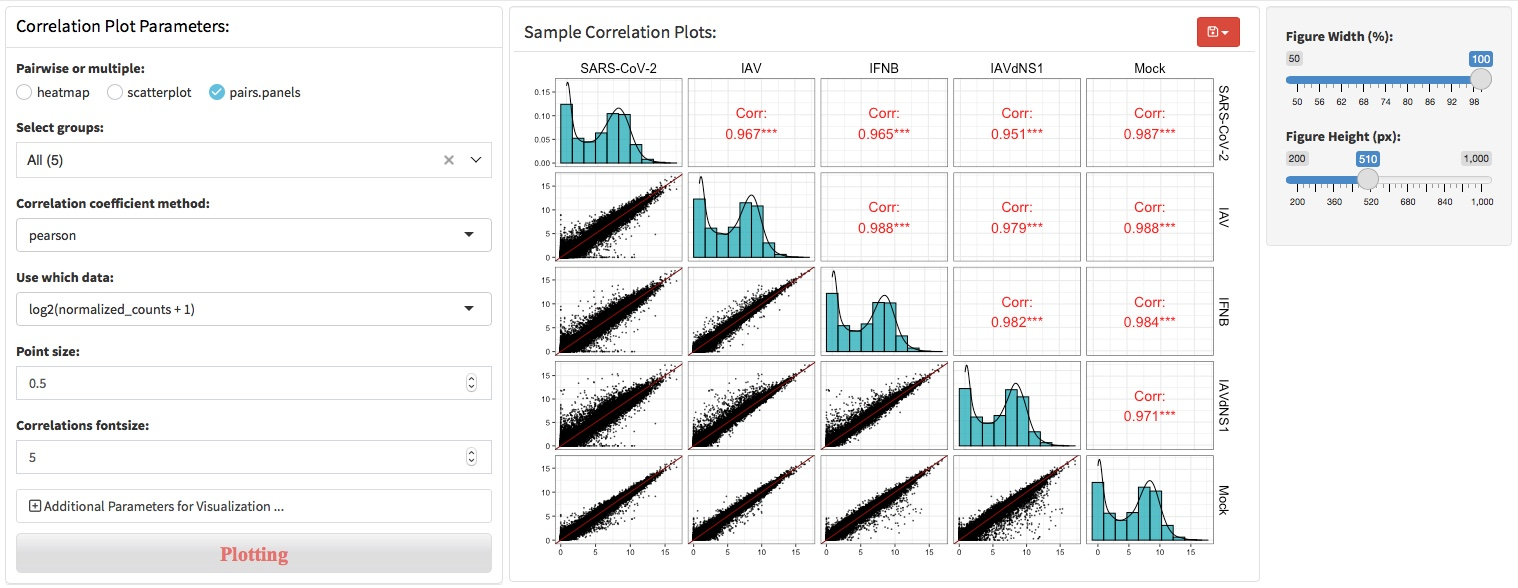
\includegraphics{images/quality_correlation-mscatter.jpeg}
\end{itemize}

\hypertarget{differential-expression-analysis}{%
\chapter{Differential expression analysis}\label{differential-expression-analysis}}

The most important application of RNA-seq is to detect differentially expressed genes between variance conditions or groups. Differential expression analysis (DEA) requires that gene expression values should be compared among samples. We chose the DESeq2 package to perform the expression normalization to adjust abundance quantities in order to account for differences in read depth across the samples. After that, the function `results' of DESeq2 wase used for calculating the foldchange of gene expression levels and P-values across experimental and control condition.

\hypertarget{extract-degs}{%
\section{Extract DEGs}\label{extract-degs}}

DESeq2 offers two kinds of hypothesis tests: the Wald test, where we use the estimated standard error of a log2 fold change to test if it is equal to zero, and the likelihood ratio test (LRT). The LRT examines two models for the counts, a full model with a certain number of terms and a reduced model, in which some of the terms of the full model are removed. The test determines if the increased likelihood of the data using the extra terms in the full model is more than expected if those extra terms are truly zero.

\hypertarget{wald-significance-tests}{%
\subsection{Wald significance tests}\label{wald-significance-tests}}

To extract DEGs, user should specify one group as control, and one or more groups as treatment. Then, the threshold of P value and log2 fold change shold be specified as well. Most commonly used standard to define differentially expressed gene (DEG) is \textbar log2FoldChange\textbar{} \textgreater{} 1 and P-value \textless{} 0.05, but we also provide the options for user's custom defined standard to filter DEGs.

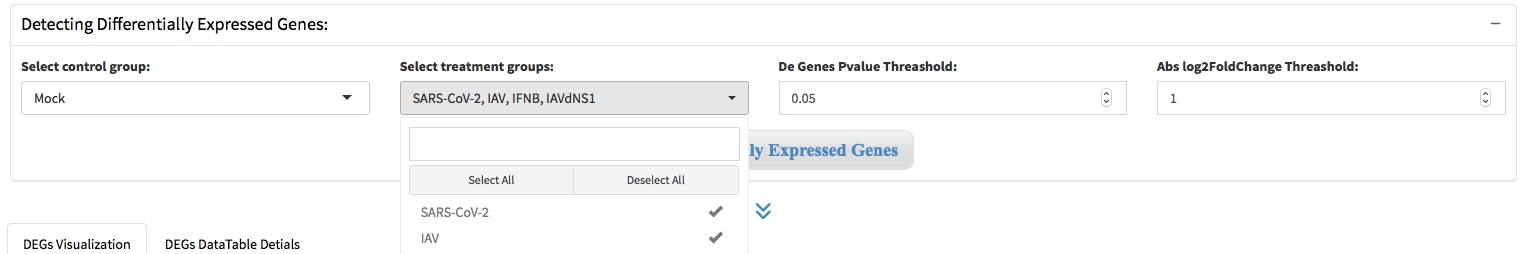
\includegraphics{images/dea-de.jpeg}

\hypertarget{likelihood-ratio-test}{%
\subsection{Likelihood ratio test}\label{likelihood-ratio-test}}

To extract DEGs by LRT, user just need to specify one group as control and one groups as treatment, cause LRT will return only one group DEGs. P-value threshold should be set no more than 0.05. Note that log2FoldChange should be set to 0.
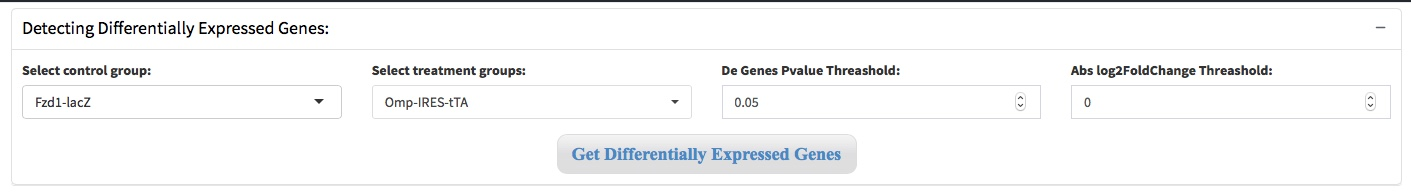
\includegraphics{images/dea-de-lrt.jpeg}

\hypertarget{visualize-degs}{%
\section{Visualize DEGs}\label{visualize-degs}}

We provide five approaches to visualize the DEGs, include volcano plot, MA-plot, bar-plot, heatmap, venn diagram.

\begin{itemize}
\item
  Volcano plot
  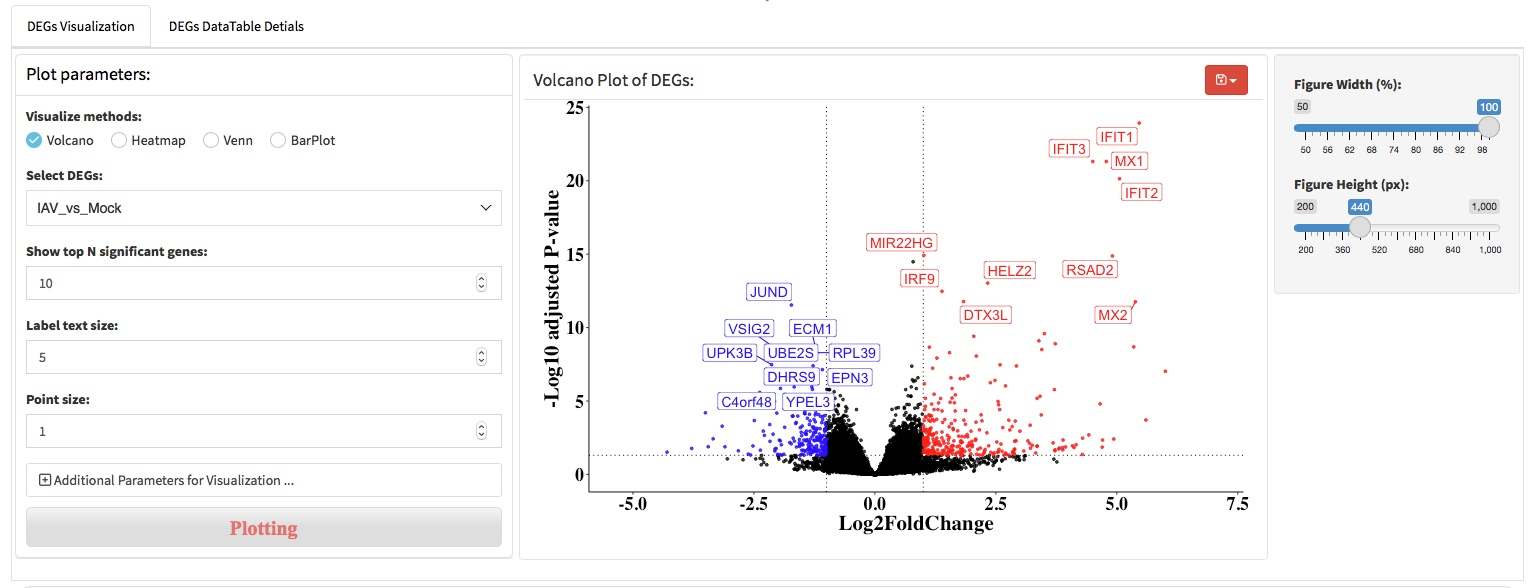
\includegraphics{images/dea-volcano.jpeg}
\item
  Heatmap
  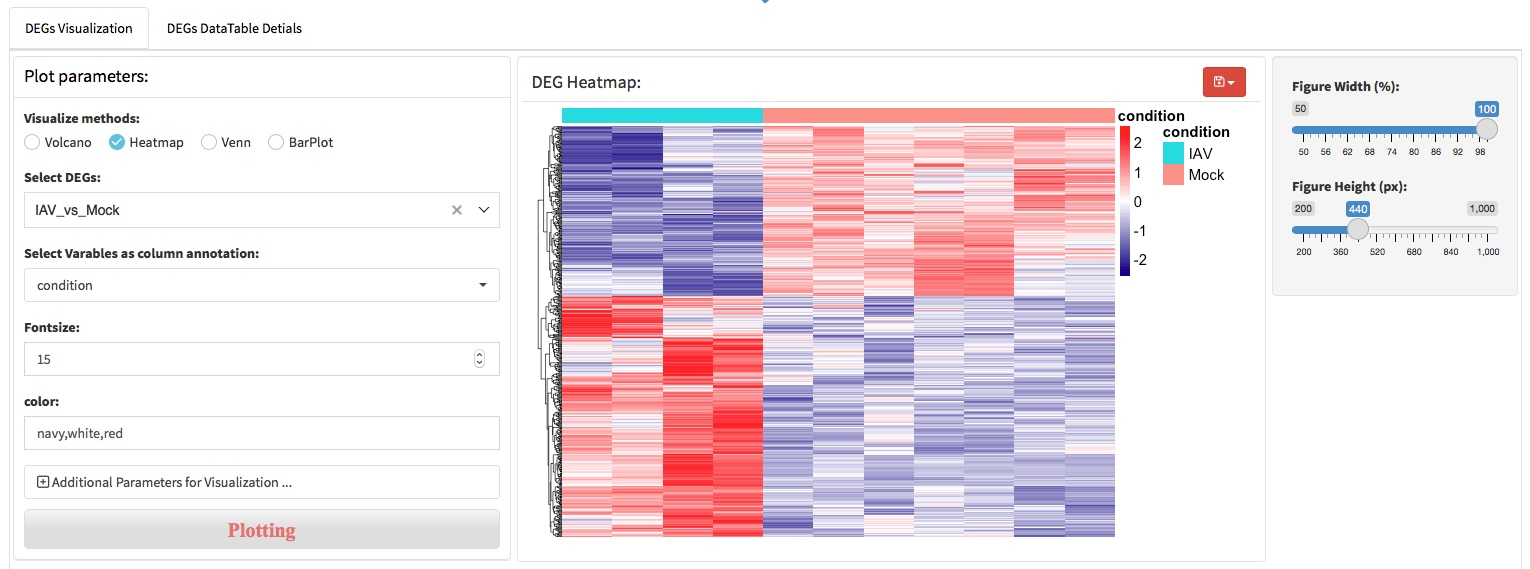
\includegraphics{images/dea-heatmap.jpeg}
\item
  Venn diagram
  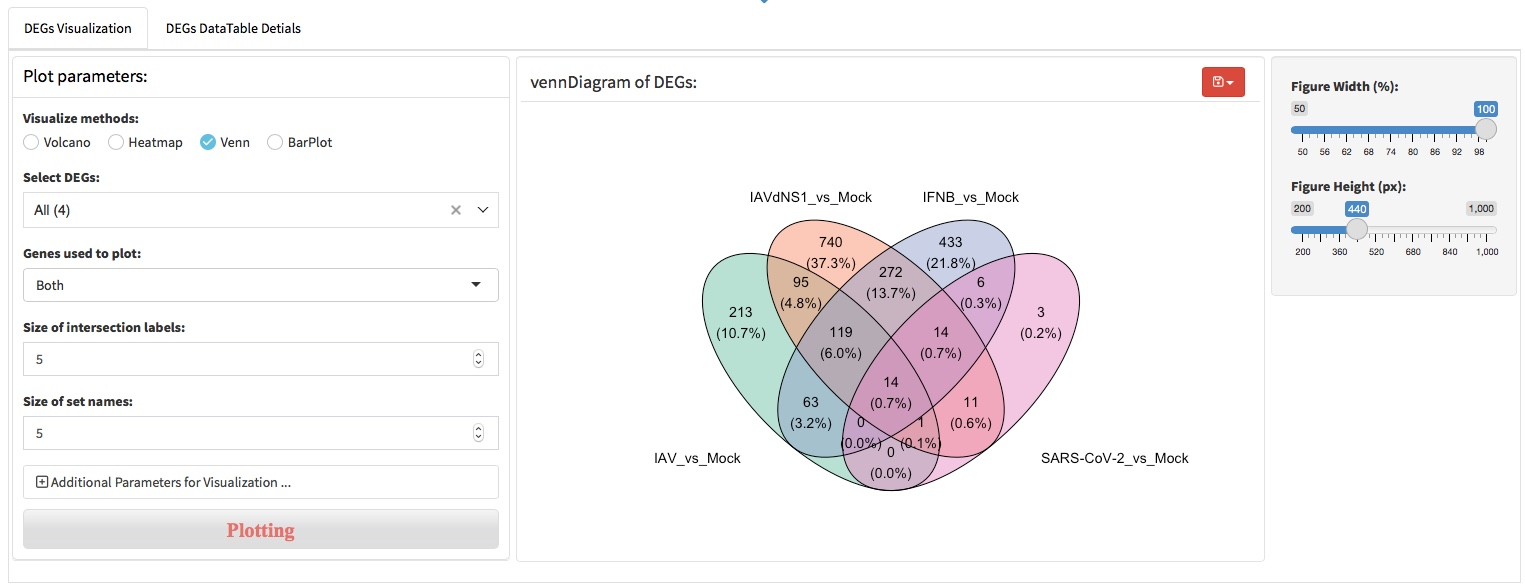
\includegraphics{images/dea-venn.jpeg}
\item
  Bar-plot
  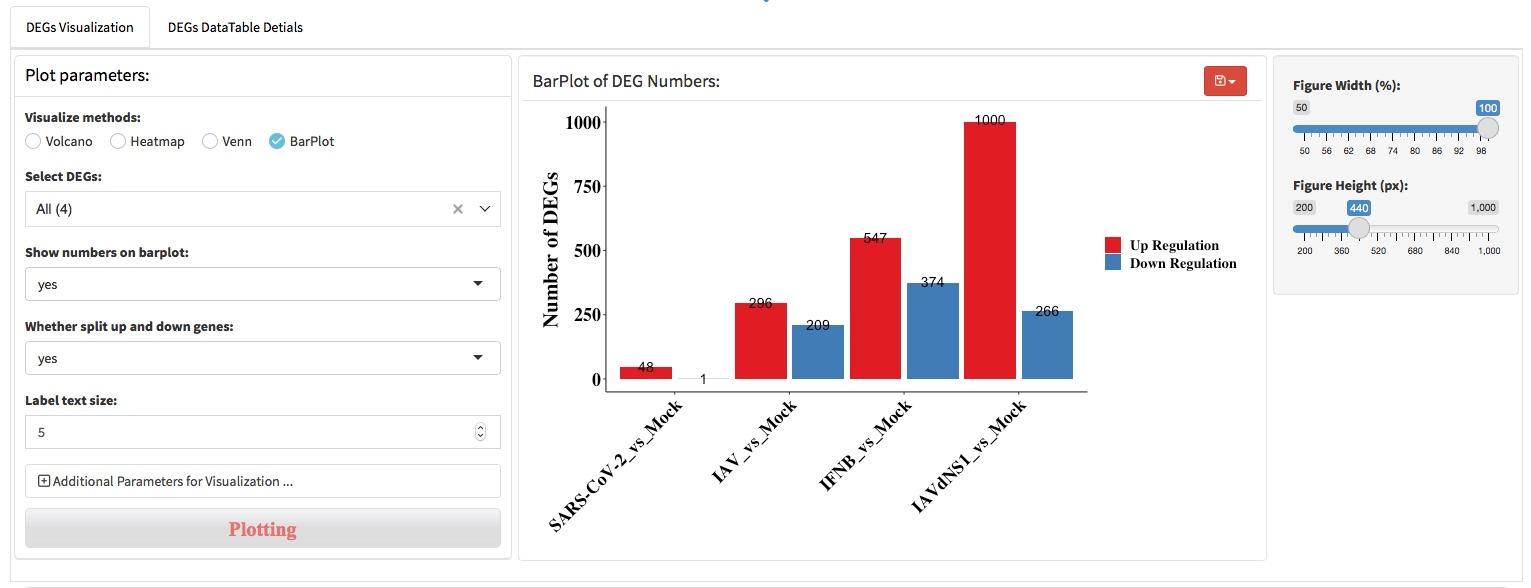
\includegraphics{images/dea-bar.jpeg}
\item
  The details of DEGs
  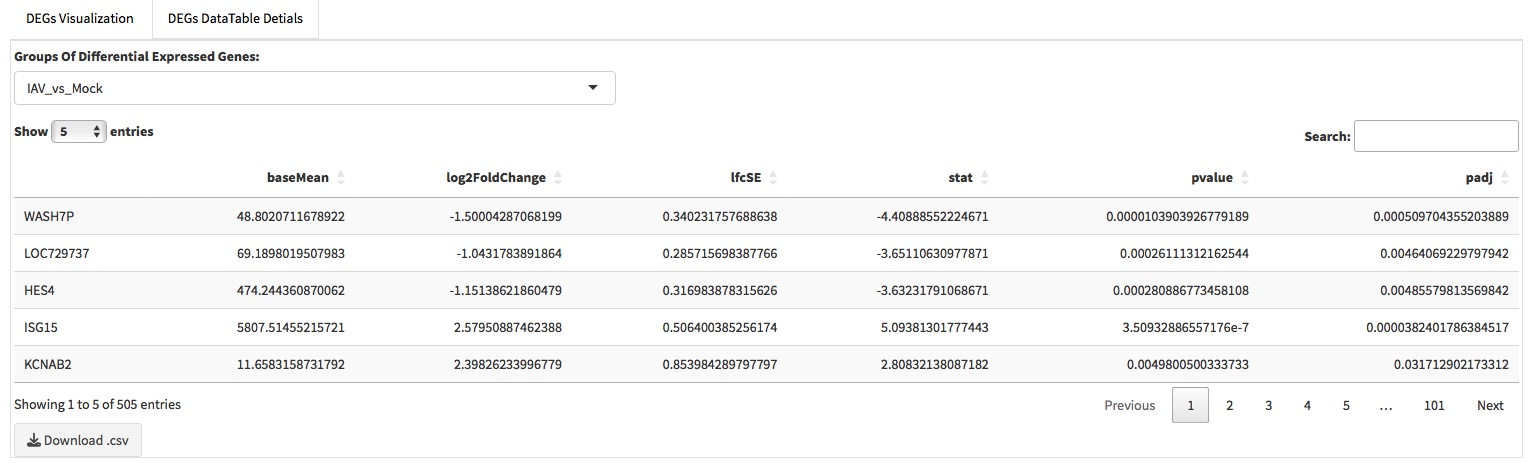
\includegraphics{images/dea-tab.jpeg}
\end{itemize}

\hypertarget{deg-expression-pattern-detection}{%
\chapter{DEG expression pattern detection}\label{deg-expression-pattern-detection}}

Research involved time series experiment would more interested in genes that differentially expressed along time points. We provide the DEGreport pacakge to distinguish different gene expression patterns of differentially expressed genes. For example, we group genes that expression increase over time into one expression pattern, and group genes that expression decrease over time into another expression pattern. These differentially expressed genes show different expression patterns over time, suggesting that they may have different biological functions and meanings.

\hypertarget{one-way-time-coures-experiment}{%
\section{One-way time coures experiment}\label{one-way-time-coures-experiment}}

\hypertarget{pre-processing-and-preparation}{%
\subsection{pre-processing and preparation}\label{pre-processing-and-preparation}}

For the time-course experiment that only the first time point was set as the control, DEGs were detected at each time point in contrast to the first time point.

\begin{itemize}
\tightlist
\item
  The condition should be time points.
  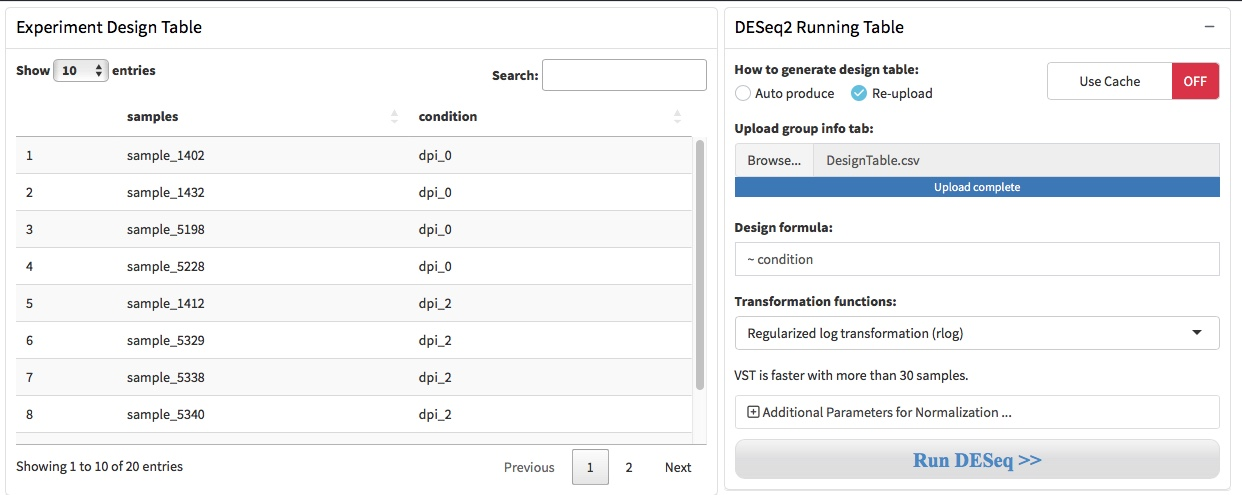
\includegraphics{images/degp_ow_designtable.jpeg}
\item
  Or using LRT to detect DEGs which at one or more time points after time 0. Set test method as ``LRT'' and reduced as ``\textasciitilde{} 1''.
  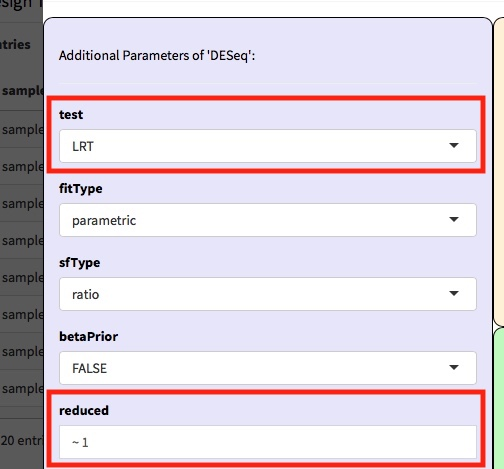
\includegraphics{images/degp_ow_designtable_lrt.jpeg}
\end{itemize}

\hypertarget{detect-deg-expression-pattern}{%
\subsection{Detect DEG expression pattern}\label{detect-deg-expression-pattern}}

Then, the DEGreport package was employed to calculate the gene similarity among samples and cluster the genes into expression patterns. To detect the DEG expression patterns, user should specify the group of DEGs, such as dpi\_2\_vs\_dpi\_0 and dpi\_4\_vs\_dpi\_0. And user need to specify the variable with which the gene expression changes. Due to there is only one time course of the experiment, thus we leave the ``variable to separate samples'' to NULL.

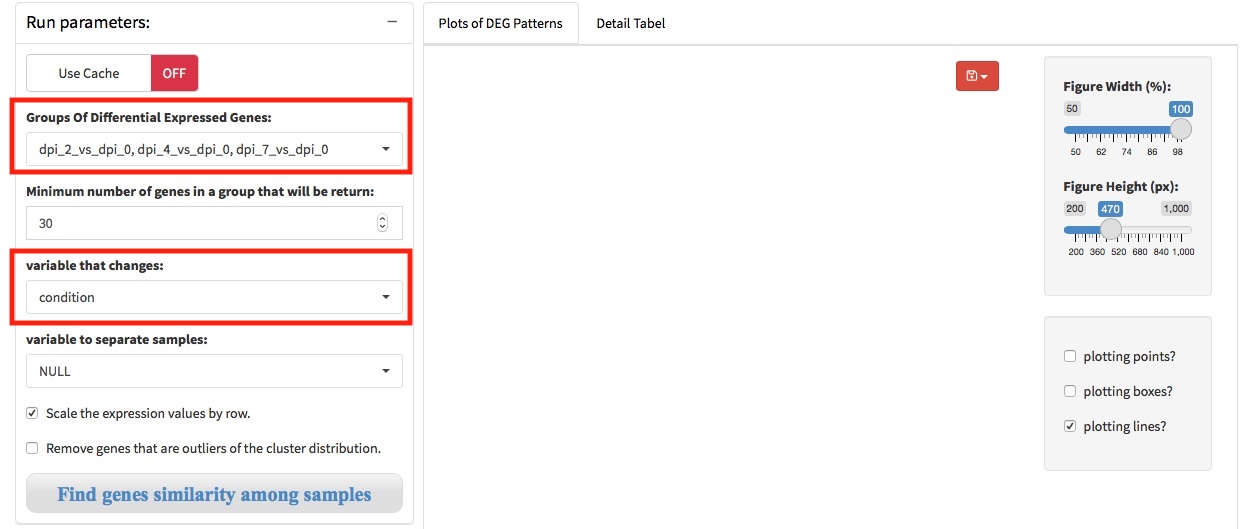
\includegraphics{images/degp_single_factor_detect.jpeg}

\hypertarget{visualize-deg-expression-pattern}{%
\subsection{Visualize DEG expression pattern}\label{visualize-deg-expression-pattern}}

User can select DEG expression pattern clusters to visualize the results, and adjust the time point order by specifing the `plotting order' option.

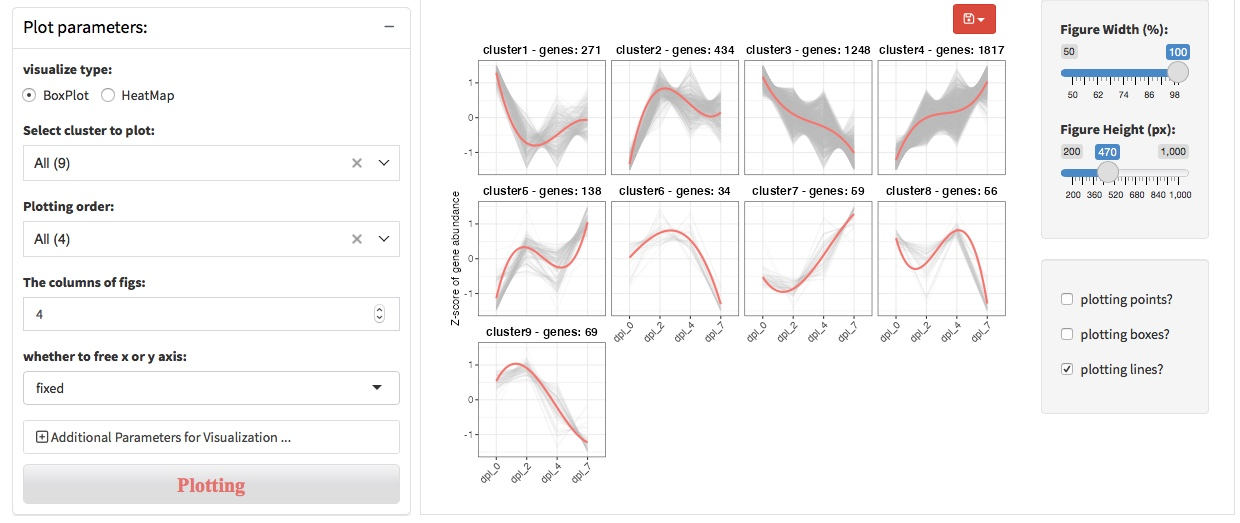
\includegraphics{images/degp_single_factor_plots.jpeg}

\hypertarget{two-way-time-coures-experiment}{%
\section{Two-way time coures experiment}\label{two-way-time-coures-experiment}}

\hypertarget{pre-processing-and-preparation-1}{%
\subsection{pre-processing and preparation}\label{pre-processing-and-preparation-1}}

For time-course experiment that sets a control at each time point, an appreciate way to detected DEGs over time is use the likelihood ratio test (LRT) with the design formula like ``\textasciitilde{} condition + time + condition:time'', and reduced formula like ``\textasciitilde{} condition + time''.

\begin{itemize}
\tightlist
\item
  set design formula as ``\textasciitilde{} condition + time + condition:time''
  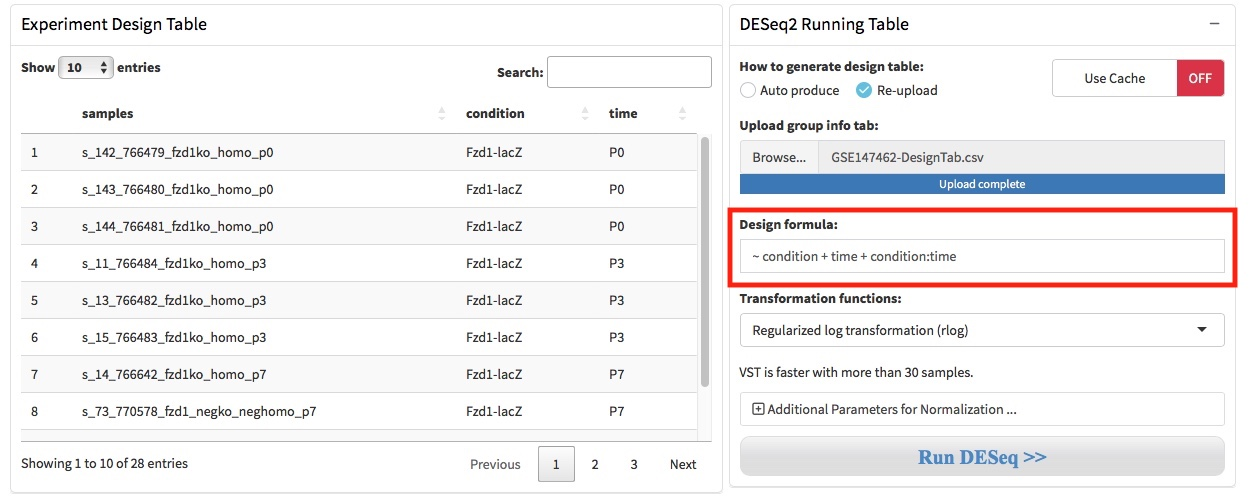
\includegraphics{images/degp_multiple_factor_design.jpeg}
\item
  set test method as ``LRT'' and reduced formula as ``\textasciitilde{} condition + time''
  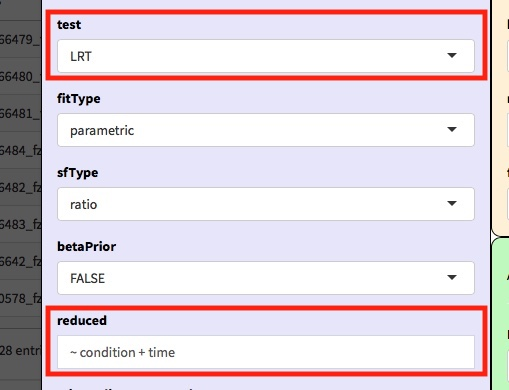
\includegraphics{images/degp_multiple_factor_adpt.jpeg}
\item
  Or detected DEGs at each time point contrast to the corresponding control in the common manner.
\end{itemize}

\hypertarget{detect-deg-expression-pattern-1}{%
\subsection{Detect DEG expression pattern}\label{detect-deg-expression-pattern-1}}

Due to there would be more than one time course of the experiment, thus we set ``variable that changes'' to ``time'' and set ``variable to separate samples'' to ``condition''.
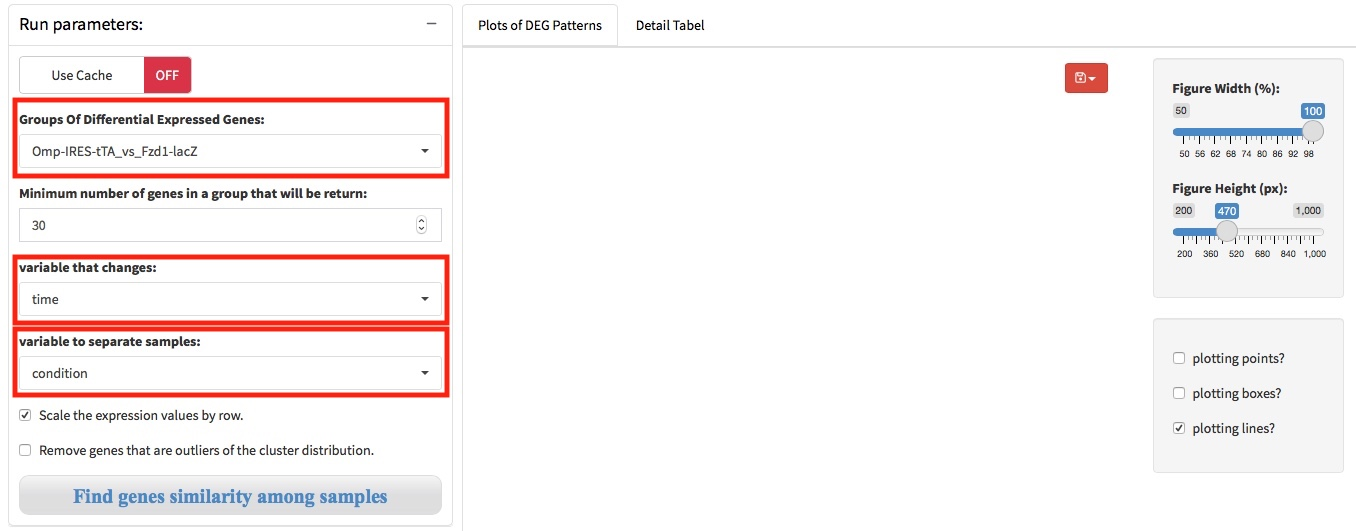
\includegraphics{images/degp_multiple_factor_detect.jpeg}

\hypertarget{visualize-deg-expression-pattern-1}{%
\subsection{Visualize DEG expression pattern}\label{visualize-deg-expression-pattern-1}}

User can select DEG expression pattern clusters to visualize the results, and adjust the time point order by specifing the `plotting order' option.

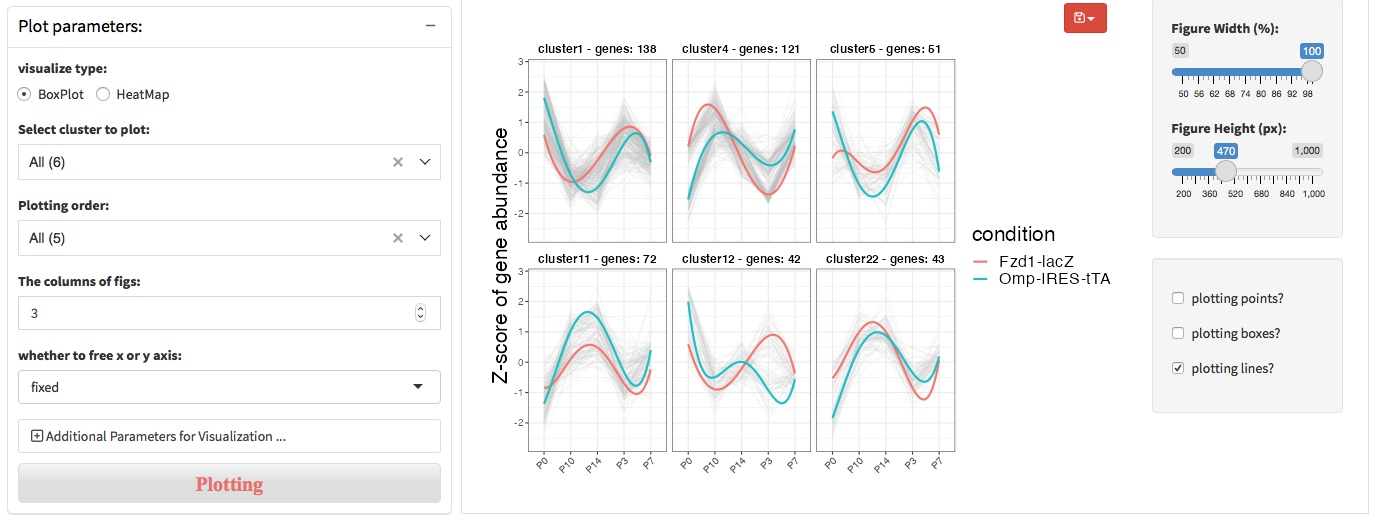
\includegraphics{images/degp_multiple_factor_plots.jpeg}

\hypertarget{weighted-correlation-network-analysis}{%
\chapter{weighted correlation network analysis}\label{weighted-correlation-network-analysis}}

We have finished a nice book.

\hypertarget{data-preparation}{%
\section{Data preparation}\label{data-preparation}}

\hypertarget{soft-threshold-detection}{%
\section{Soft threshold detection}\label{soft-threshold-detection}}

\hypertarget{gene-module-detection}{%
\section{Gene module detection}\label{gene-module-detection}}

\hypertarget{module-traits-relationship}{%
\section{Module-Traits relationship}\label{module-traits-relationship}}

\hypertarget{mm-vs.-gs-scatterplot}{%
\section{MM vs.~GS scatterplot}\label{mm-vs.-gs-scatterplot}}

\hypertarget{module-gene-expression-visualization}{%
\section{Module gene expression visualization}\label{module-gene-expression-visualization}}

\hypertarget{functional-enrichment-analysis}{%
\chapter{functional enrichment analysis}\label{functional-enrichment-analysis}}

After the differential expression analysis and biological pattern detection (DEG patterns and WGCNA modules), functional enrichment analysis was usually used to characterize the molecular functions or pathways in which genes involved. There are two main approaches to perform the functional enrichment analysis, (i) ORA that using a list of genes of interest as input and (ii) GSEA that using all genes ranked by log2foldchange as input. We apply clusterProfiler and gprofiler2 (an R client of g:Profiler) to perform the ORA and GSEA analysis. In addition to supporting the use of Gene Ontology, KEGG, and Reactome knowledge base, gprofiler2 also support WikiPathway, miRTarBase, TRANSFAC, Human Protein Atlas, CORUM and Human Phenotype Ontology knowledge base.

\hypertarget{gprofiler-api}{%
\section{Gprofiler API}\label{gprofiler-api}}

g:Profiler is a public web server for characterising and manipulating gene lists. The R package gprofiler2 provides an R interface to the g:Profiler tools. g:Profiler is developed and maintained in Estonia, at the University of Tartu, Institute of Computer Science, Bioinformatics, Algorithmics and Data Mining Group BIIT. Currently g:Profiler is developed and maintained by a team of professional software developers, statistician and researchers.

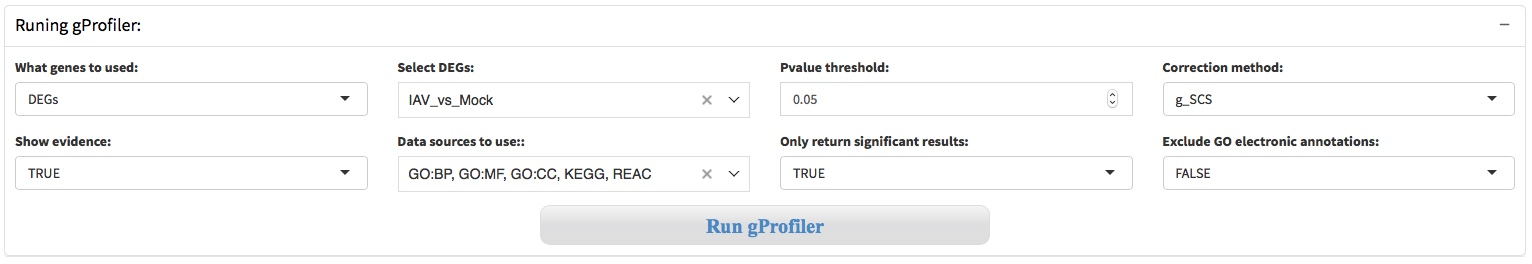
\includegraphics{images/fucntion-grofiler.jpeg}

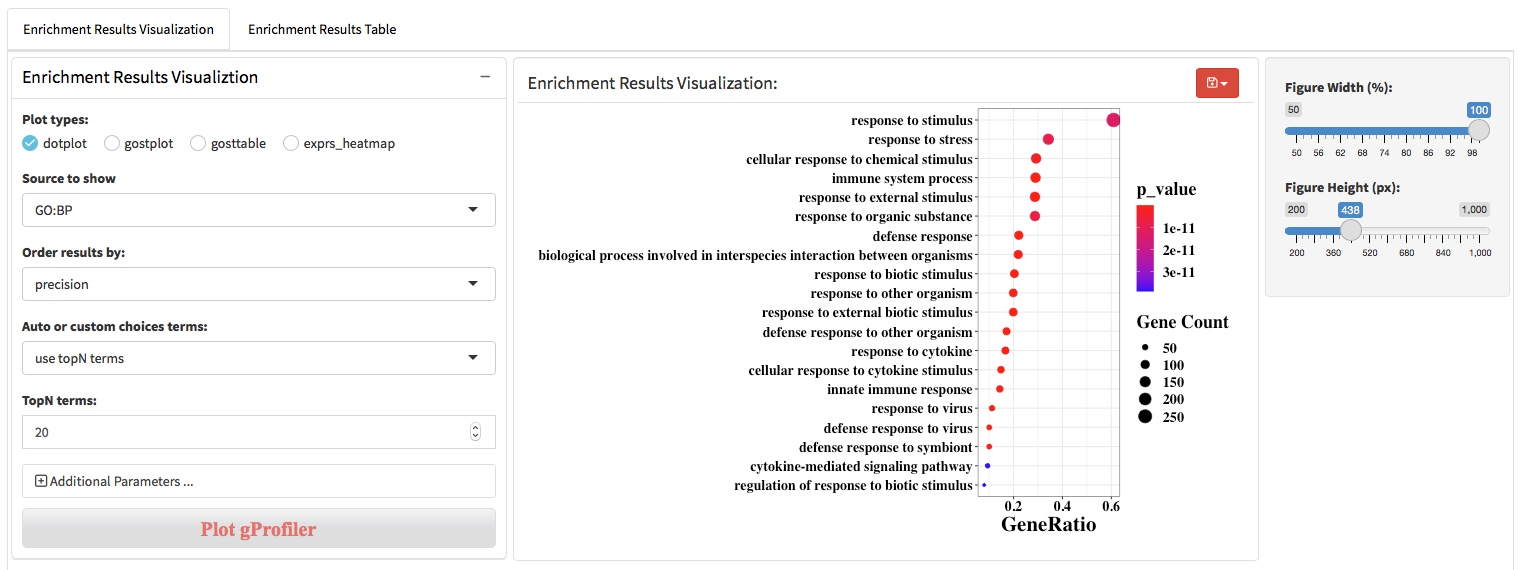
\includegraphics{images/fucntion-grofiler-dot.jpeg}

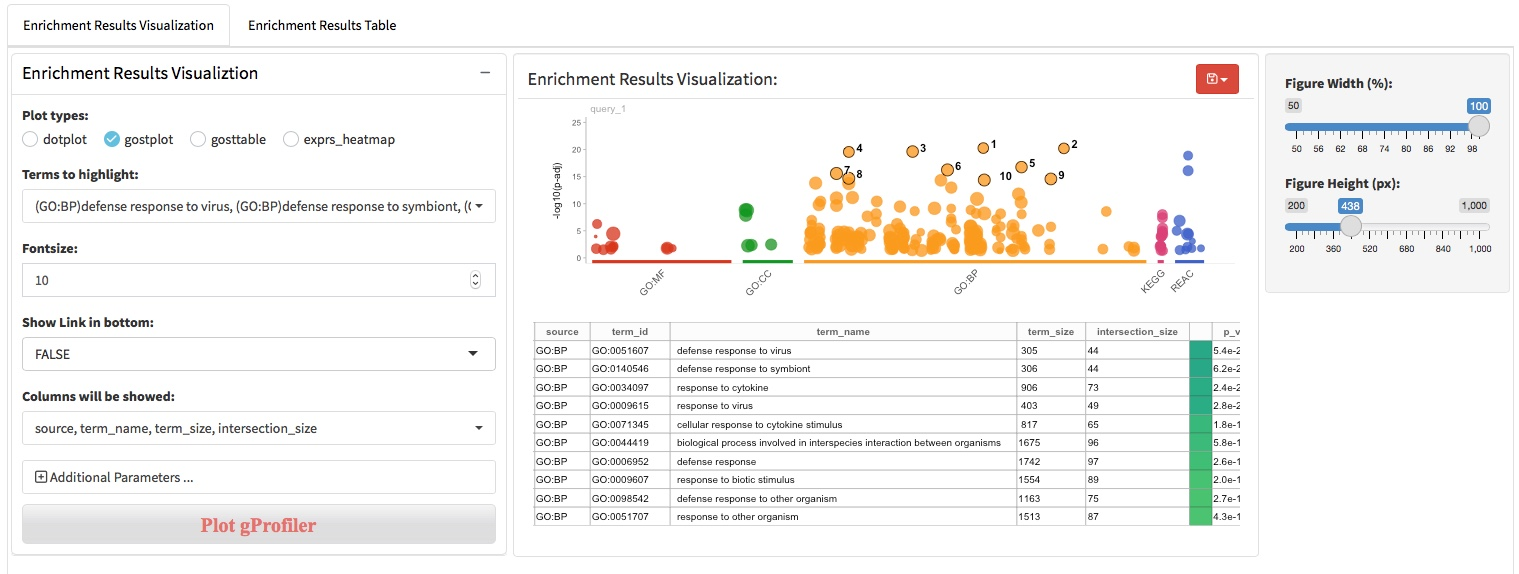
\includegraphics{images/fucntion-grofiler-gostdot.jpeg}

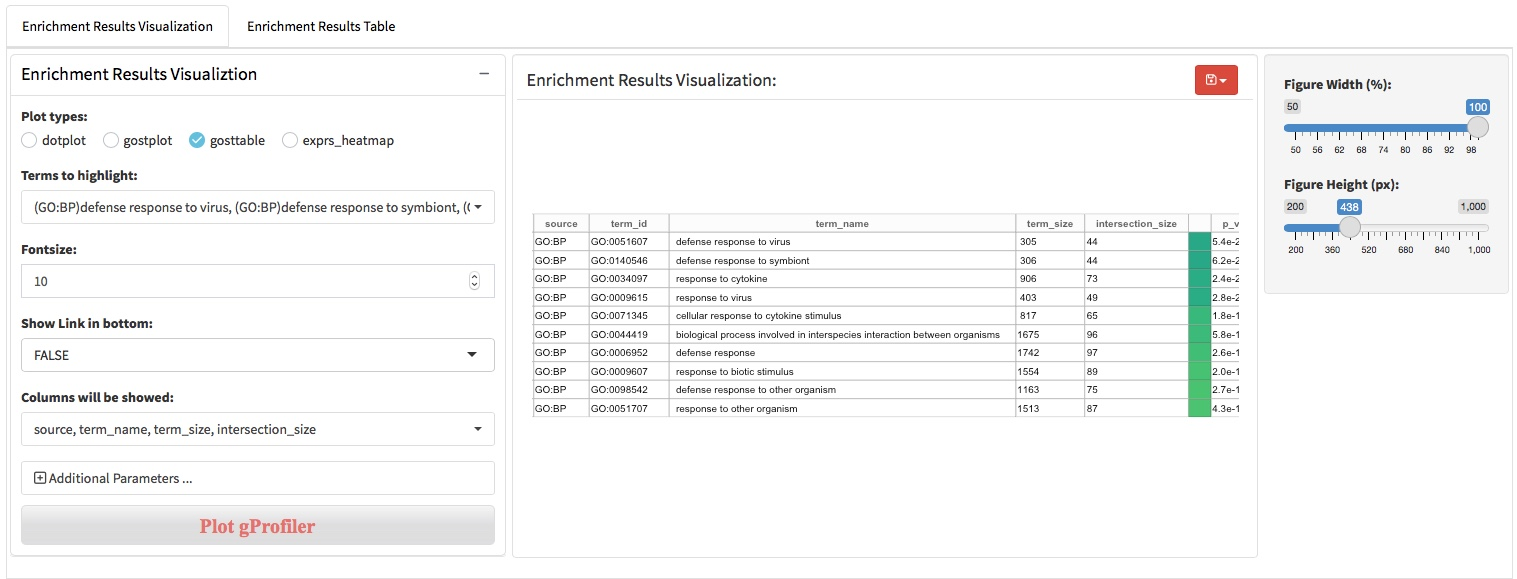
\includegraphics{images/fucntion-grofiler-gosttab.jpeg}

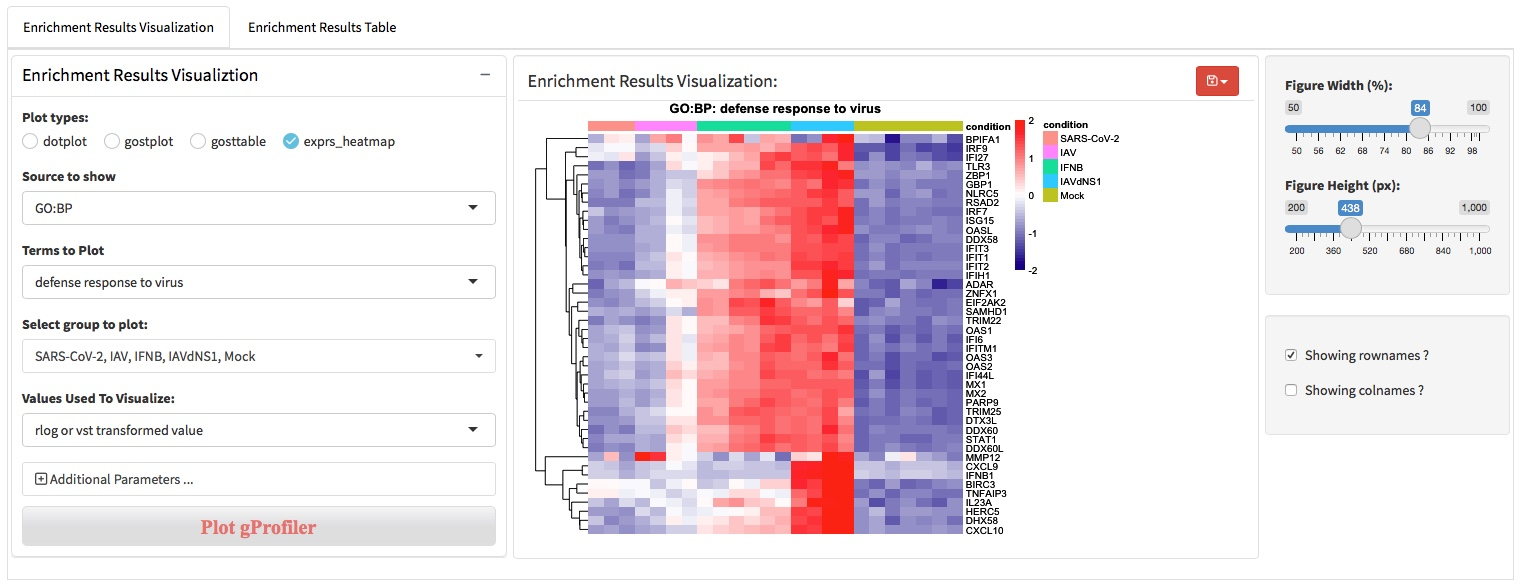
\includegraphics{images/fucntion-grofiler-heatmap.jpeg}

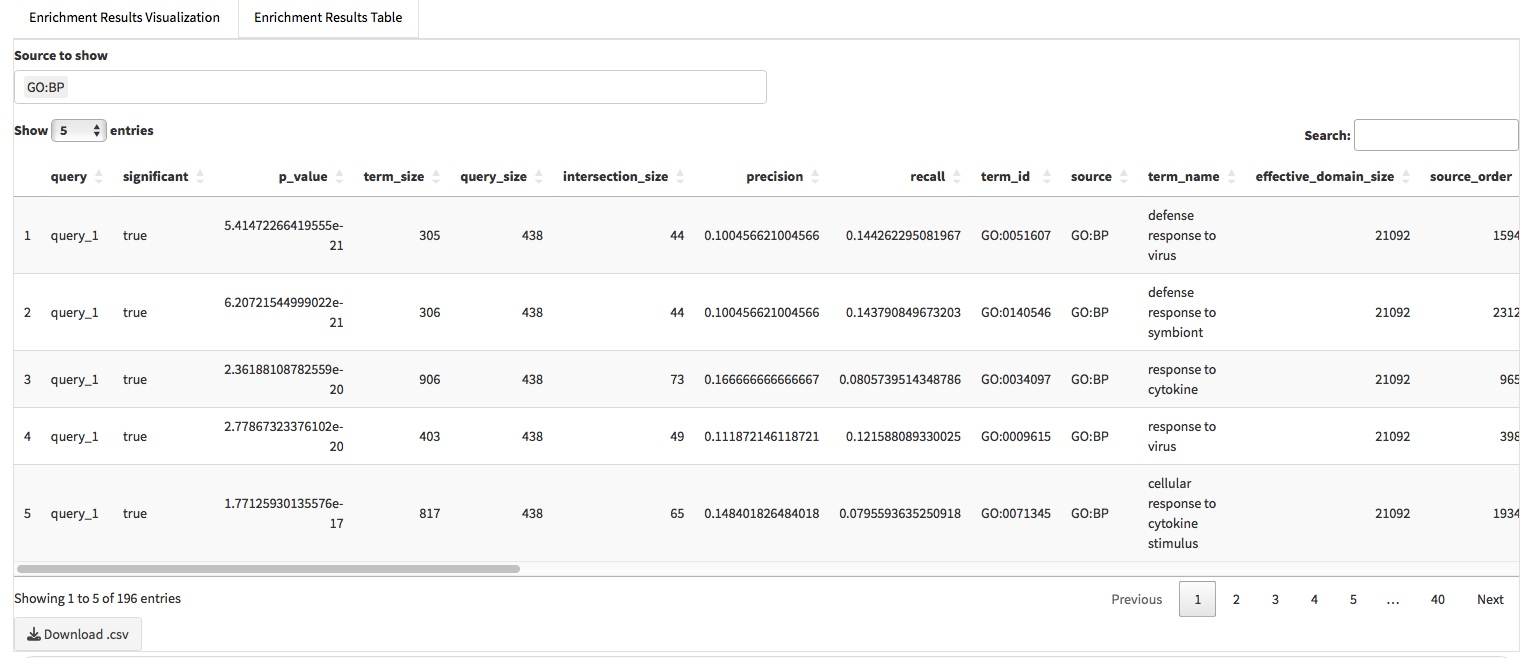
\includegraphics{images/fucntion-grofiler-tab.jpeg}

\hypertarget{clusterprofiler-ora}{%
\section{ClusterProfiler-ORA}\label{clusterprofiler-ora}}

\hypertarget{clusterprofiler-gsea}{%
\section{ClusterProfiler-GSEA}\label{clusterprofiler-gsea}}

\hypertarget{gene-regulatory-network}{%
\chapter{Gene regulatory network}\label{gene-regulatory-network}}

We have finished a nice book.

\hypertarget{kegg-pathview}{%
\section{KEGG Pathview}\label{kegg-pathview}}

\hypertarget{ppi-network}{%
\section{PPI network}\label{ppi-network}}

\hypertarget{genie3-inffered-network}{%
\section{GENIE3 inffered network}\label{genie3-inffered-network}}

\hypertarget{summary-of-genes-and-functions}{%
\chapter{Summary of genes and functions}\label{summary-of-genes-and-functions}}

We have finished a nice book.

\hypertarget{summarize-genes}{%
\section{summarize genes}\label{summarize-genes}}

\hypertarget{summarize-functions}{%
\section{summarize functions}\label{summarize-functions}}

  \bibliography{book.bib,packages.bib}

\end{document}
